\documentclass[3p]{elsarticle}

\usepackage{lineno,hyperref}
\modulolinenumbers[5]

\usepackage{amsmath, amssymb}
\usepackage[bbgreekl]{mathbbol}
\usepackage{subfigure}
\usepackage{wrapfig}
\usepackage{enumerate}
\usepackage{bm}
\usepackage{color}
\usepackage{multirow}

\makeatletter 
  \newcommand\figcaption{\def\@captype{figure}\caption} 
  \newcommand\tabcaption{\def\@captype{table}\caption} 
\makeatother

\journal{Computer Aided Geometric Design}

%%%%%%%%%%%%%%%%%%%%%%%
%% Elsevier bibliography styles
%%%%%%%%%%%%%%%%%%%%%%%
%% To change the style, put a % in front of the second line of the current style and
%% remove the % from the second line of the style you would like to use.
%%%%%%%%%%%%%%%%%%%%%%%

%% Numbered
%\bibliographystyle{model1-num-names}

%% Numbered without titles
%\bibliographystyle{model1a-num-names}

%% Harvard
%\bibliographystyle{model2-names.bst}\biboptions{authoryear}

%% Vancouver numbered
%\usepackage{numcompress}\bibliographystyle{model3-num-names}

%% Vancouver name/year
%\usepackage{numcompress}\bibliographystyle{model4-names}\biboptions{authoryear}

%% APA style
%\bibliographystyle{model5-names}\biboptions{authoryear}

%% AMA style
%\usepackage{numcompress}\bibliographystyle{model6-num-names}

%% `Elsevier LaTeX' style
\bibliographystyle{elsarticle-num}
%%%%%%%%%%%%%%%%%%%%%%%

\begin{document}


\begin{frontmatter}

\title{GPU-based Smooth Free-Form Deformation with Sharp Feature Awareness}
%\tnotetext[mytitlenote]{Fully documented templates are available in the elsarticle package on \href{http://www.ctan.org/tex-archive/macros/latex/contrib/elsarticle}{CTAN}.}

%% Group authors per affiliation:
%\author{Elsevier\fnref{myfootnote}}
%\address{Radarweg 29, Amsterdam}
%\fntext[myfootnote]{Since 1880.}

%% or include affiliations in footnotes:
%\author[mymainaddress,mysecondaryaddress]{Elsevier Inc}
%\ead[url]{www.elsevier.com}

%\author[mysecondaryaddress]{Global Customer Service\corref{mycorrespondingauthor}}
%\cortext[mycorrespondingauthor]{Corresponding author}
%\ead{support@elsevier.com}

%\address[mymainaddress]{1600 John F Kennedy Boulevard, Philadelphia}
%\address[mysecondaryaddress]{360 Park Avenue South, New York}

%%%%%%%%%%%%%%%%%%%%%%%%%%%%%%%%%%%%%%%%%%
\author{Yuanmin Cui}

\author{Jieqing Feng\corref{mycorrespondingauthor}}
\cortext[mycorrespondingauthor]{Corresponding author}
\ead{jqfeng@cad.zju.edu.cn}

\address{State Key Lab of CAD\&CG, Zhejiang University, China}
%%%%%%%%%%%%%%%%%%%%%%%%%%%%%%%%%%%%%%%%%%

\begin{abstract}
In an accurate free-form deformation of a polygonal object, only the linear geometry, e.g., triangles or planar
polygons, is deformed as triangular B\'ezier patches or trimmed tensor product B\'ezier patches; the related normal
field is not considered. Thus, the geometry appearance and shading of the deformed object are typically not smooth. In
this paper, both the linear geometry and normal of a polygonal object are simultaneously considered in the framework of
accurate free-form deformation. First, each triangle and its normal field are deformed as two cubic triangular B\'ezier
patches. Then, the curved geometry corresponding to the deformed triangles is locally adjusted to tone the smoothness of
the geometry appearance according to the deformed normal field. The deformed normal field is adjusted accordingly. As a
result, a smooth free-form deformation with visually plausible smooth geometry and shading is obtained. Furthermore,
the sharp features in the polygonal object can be preserved. Because the curved geometry and normal field adjustments
are local operations, all of the above computations can be performed in parallel on a GPU. The experimental results
show that the method can deform a complex polygonal object as a smooth object in real time while preserving sharp
features.
\end{abstract}

\begin{keyword}
%\texttt{elsarticle.cls}\sep \LaTeX\sep Elsevier \sep template
smooth FFD\sep sharp feature preserving\sep GPU\sep \textcolor{red}{cubic triangular B\'ezier patch\sep normal field}
%\MSC[2010] 00-01\sep  99-00
\end{keyword}

\end{frontmatter}

\linenumbers

\section{Introduction}

Free-form deformation (FFD) is a prevalent shape manipulation and shape animation method in computer graphics and
geometric modeling~\cite{Sederberg86}. Classic FFD is conducted on the sampled points of the geometric model. However,
the approach tends to produce an aliased deformation result when using a low sampling density.

As an alternative, accurate FFD~\cite{Feng98, Feng02, Feng00} deforms the planar polygons as a set of triangular
B\'ezier patches or trimmed tensor-product B\'ezier patches based on the functional composition of Bernstein
polynomials~\cite{DeRose88, DeRose93}. The deformation result is accurate for polygonal objects in theory. The accurate
FFD considers only the geometry of the original model, excluding its normal field. As a result, the deformed object is
only \textcolor{red}{position} continuous \textcolor{red}{$(C^0)$} for its geometry. Its geometric appearance (e.g.,
silhouettes and the common edge of two patches) and shading are not smooth because the normal field is
\textcolor{red}{discontinuous.}

In mathematics, the normal is a differential attribute of the surface. In many graphics applications, the geometry and
normal of a polygonal object are independently defined. Each vertex is equipped with one or more normals. In general,
the independent normal is an approximation of the potentially true normal. The sharp features, such as sharp edges and
corners, can also be preserved by assigning several normals to one vertex. For example, Phong shading can achieve smooth
shading \textcolor{red}{effect} at a low computational cost via linear normal interpolation across a triangle. To
alleviate the unsmooth silhouette problem in Phong shading, the PN-triangle~\cite{Vlachos01} method and Phong
tessellation~\cite{Boubekeur08} method alter the linear geometry of a triangle as a curved geometry according to the
related normal field.

In this paper, a new GPU-based smooth FFD with sharp feature awareness is proposed for polygonal objects in the
framework of accurate FFD, where both the geometry and normal are simultaneously considered. The deformations of the
linear geometry (triangle) and linear normal field defined on the triangles are approximated as two cubic triangular
B\'ezier patches for efficiency. As a result, the geometry appearance and shading of the deformed objects are visually
plausible smooth, and the sharp features can also be well preserved. Figure~\ref{fig:all_ffd} shows examples of various
FFD results. The main contributions of the paper are summarized as follows:

\begin{itemize}
	\item Both the linear geometry and its normal field are considered in the framework of accurate FFD.
	\item \textcolor{red}{The deformed object exhibits a continuous shading mimicking a $G^1$ surface over smooth edges
		(implemented as $C^0$ normal field over a $C^0$ geometry), while sharp edges exhibit a discontinuous normal field.}
	\item All of the computations are local and can be implemented fully in parallel on a GPU.
\end{itemize}

\begin{figure}[htb]
	\centering
	\subfigure[Flat shading]{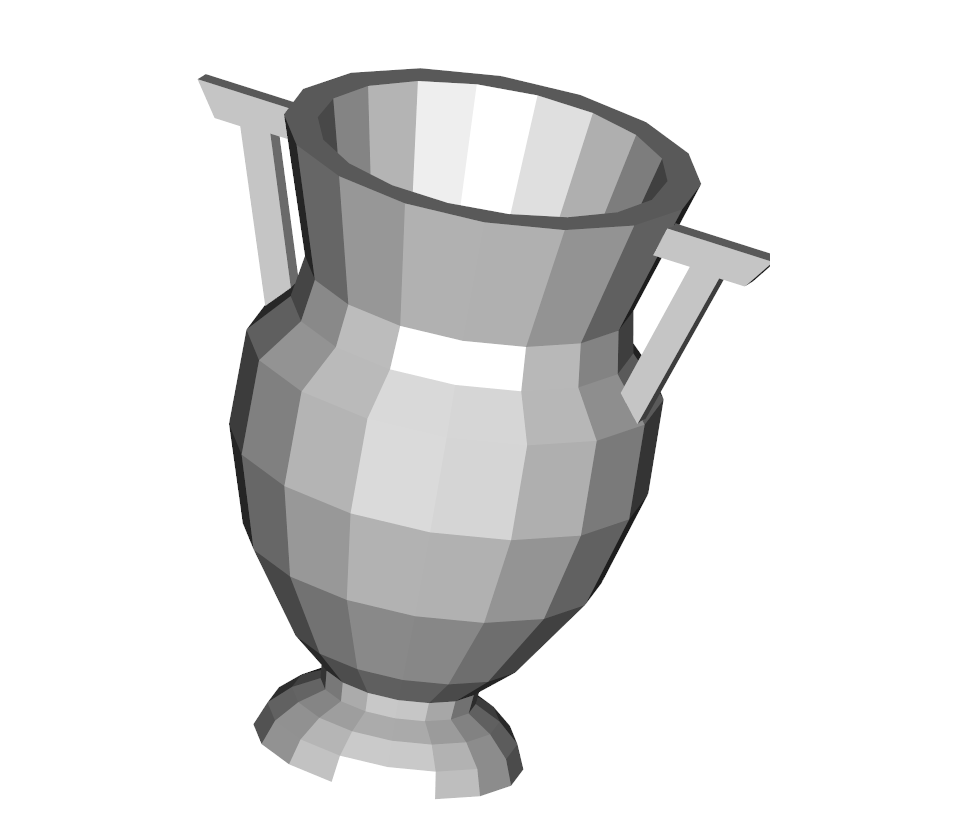
\includegraphics[width=0.17\linewidth]{pic/all_ffd_1.png}}
	\subfigure[Phong shading]{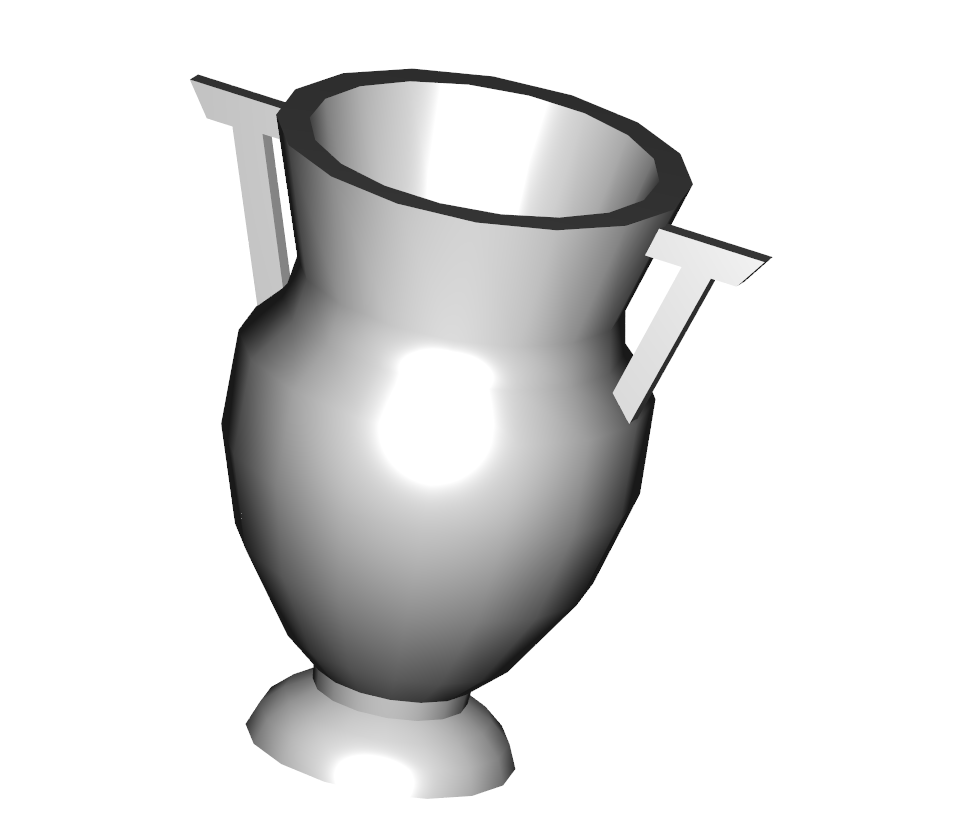
\includegraphics[width=0.17\linewidth]{pic/all_ffd_2.png}}
	\subfigure[Classic FFD]{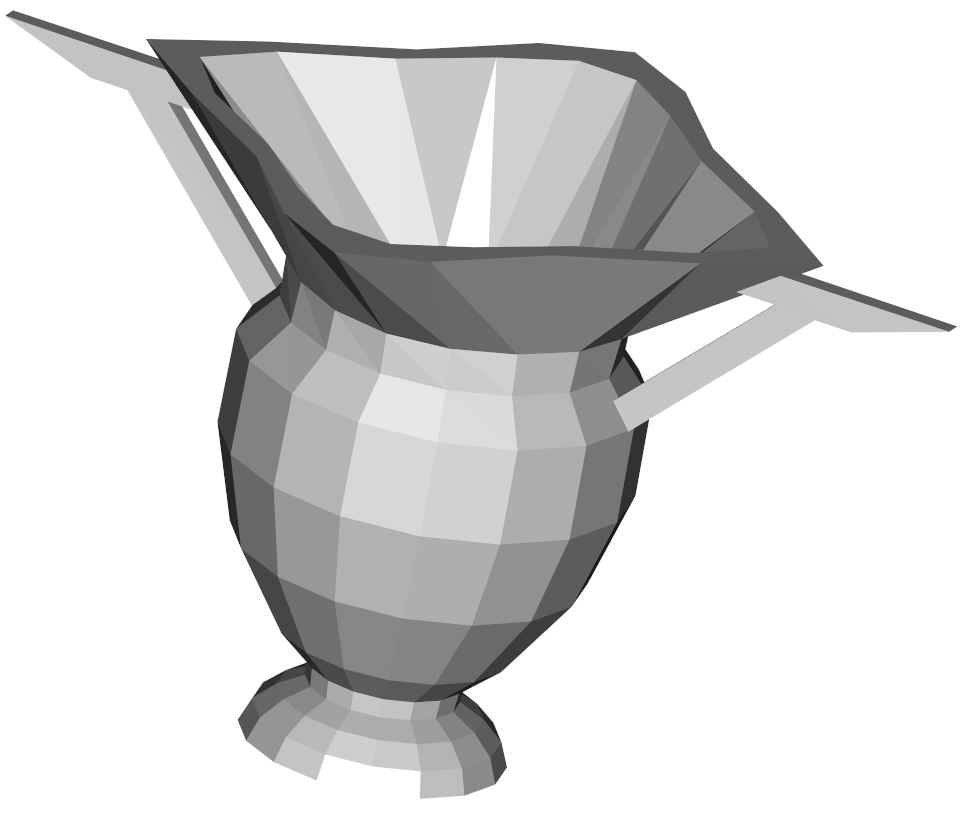
\includegraphics[width=0.17\linewidth]{pic/all_ffd_3.png}}
	\subfigure[Accurate FFD]{\label{fig:all_ffd:d}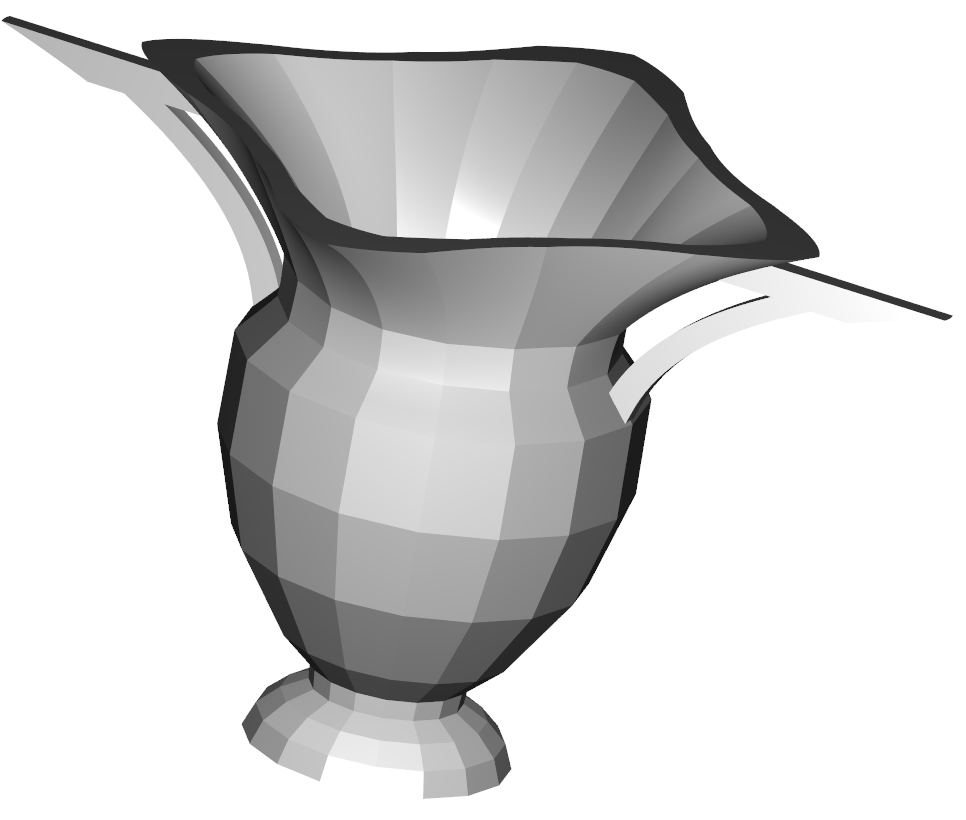
\includegraphics[width=0.17\linewidth]{pic/all_ffd_4.png}}
	\subfigure[Smooth FFD]{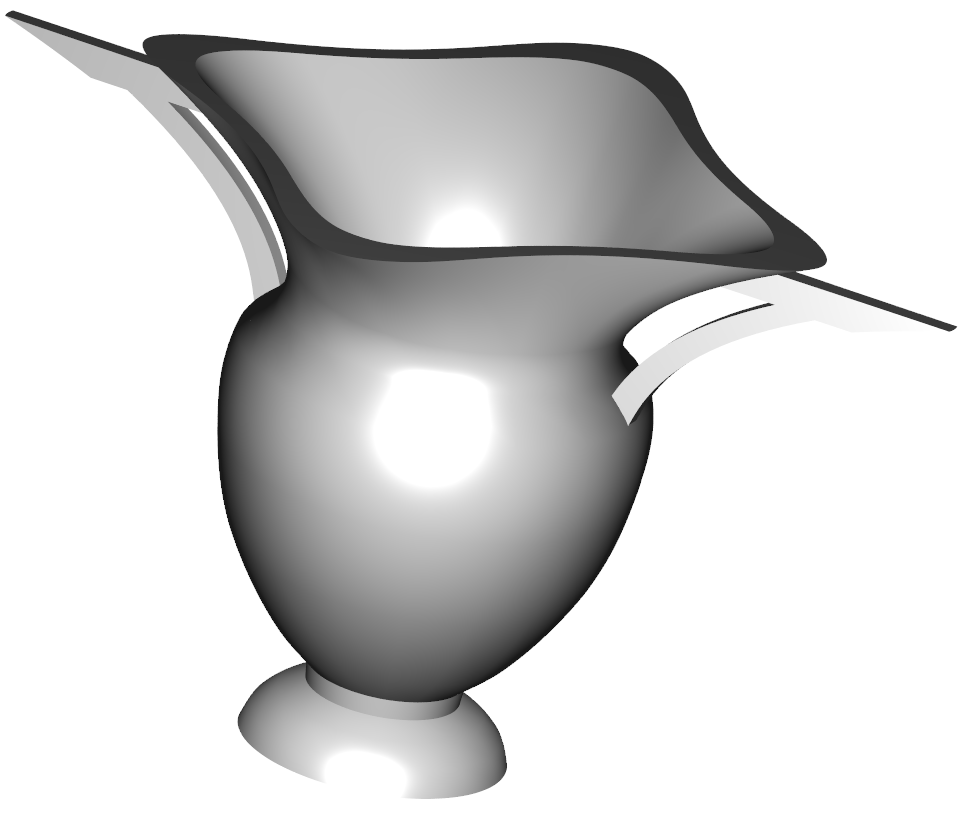
\includegraphics[width=0.17\linewidth]{pic/all_ffd_5.png}}
	\caption{Examples of classic FFD, accurate FFD and smooth FFD}
	\label{fig:all_ffd}
\end{figure}



%%%%%%%%%%%%%%%%%%%%%%%%%%%%%%%%%%%%%%%%%%%%%%%%%%%%%%%%%%%%%%%%%%%%

\section{Related Work}\label{sec:related}

FFD, which was first proposed by Sederberg and Parry~\cite{Sederberg86}, is an intuitive model manipulation and soft
object animation method. The main concept of FFD is to embed the object into an intermediate space, e.g., a B\'ezier
volume. Users first edit the shape of the intermediate space; then, the space deformation is transferred to the embedded
object, whereas the topological connectivity of the object remains unchanged. There are many successive studies
regarding FFD. Most of these studies focus on improving the interactive means of FFD \cite{Coquillart90, Hui02,
MacCracken96, McDonnel07, Xu13}. Gain and Bechmann~\cite{Gain08} provided a detailed survey of these methods.

Traditional FFD and its extensions deform the sampled vertices of the model. Thus, the quality of the deformation result
depends on the sampling density of the vertex. As a solution to the sampling problem, adaptive upsampling approaches
\cite{Gain99, Griessmair89, Parry86} are more efficient than the naive uniform upsampling approach on CPU. The adaptive
upsampling approaches consider the polygon size or surface curvature and upsample the model if necessary. But they
cannot handle certain special or pathological cases well, and are difficult to be ported on GPU. Accurate FFD, which
was proposed by Feng et al.~\cite{Feng98, Feng02, Feng00}, is an alternative approach to solving the sampling problem.
However, it is computationally intensive, and it also consumes considerable bandwidth, i.e., transferring a large amount
of data from the CPU to the GPU after the intensive computations are performed in the CPU. Thus, the algorithms are not
interactive or performed in real time in practical applications.

In the recent years, GPUs have been widely adopted for FFD implementations due to their tremendous parallel computing
power. Chua et al.~\cite{Chua00} proposed an OpenGL-oriented hardware evaluator sub-system to accelerate FFD
evaluations. However, none of the GPU vendors integrate this type of dedicated sub-system into their GPUs. In contrast,
GPUs have evolved into general-purpose many-core processors. Schein et al.~\cite{Schein06} implemented a GPU-accelerated
FFD using the NVIDIA CG language. Jung et al.~\cite{Jung11} achieved the same goal using NVIDIA CUDA and embedded it to
the X3D system. Hahmann et al.~\cite{Hahmann12} proposed a GPU-based, volume-preserving FFD. They employed the
multilinear property of volume constraint and derived an explicit solution. The GPU acceleration component implemented
by CUDA is 6.5-times faster than its CPU counterpart.

Cui et al.~\cite{Cui13, Cui14} proposed GPU-based accurate FFD of polygonal objects, the results of which are
represented in terms of trimmed tensor product B\'ezier patches or triangular B\'ezier patches. They are sufficiently
efficient to meet the real-time or interactive demands of large-scale models. However, the deformation is only performed
on the linear geometry, without considering the normal of the model. The actual normal of the resulting B\'ezier patch
is adopted for rendering. Due to the piecewise linear continuity of the polygonal object, the deformed object is only
\textcolor{red}{$C^0$} continuous. As a result, both the geometric appearance and shading effect are unsmooth. The PN-triangle
method~\cite{Vlachos01} decouples the linear geometry and normal information of a polygonal object to achieve visually
plausible smooth geometry and shading, in which it adopts cubic and quadratic triangular B\'ezier surfaces to represent
the geometry and normal, respectively. Phong tessellation \cite{Boubekeur08} proposed by Boubekeur et al. uses scalar
tags to solve the sharp edge problem. The decoupled approaches inspired us to propose a novel method to address the
above smoothness problem in the accurate FFD of polygonal objects.

%%%%%%%%%%%%%%%%%%%%%%%%%%%%%%%%%%%%%%%%%%%%%%%%%%%%%%%%%%%%%%%%%%%%

\section{Overview of Accurate FFD in Terms of Triangular B\'ezier Patches}

The GPU-based accurate FFDs~\cite{Cui13, Cui14} of polygonal objects adopt trimmed tensor product B\'ezier patches and
triangular B\'ezier patches as the deformation result, respectively. In this paper, we adopt the framework of accurate
FFD using triangular B\'ezier patches~\cite{Feng98, Feng00, Cui14} since it is more efficient than the one using trimmed
tensor product B\'ezier patches. Some basic notation is introduced below.

$\mathbf R(u,v,w)$ is a B-spline volume of degree $n_u\times n_v\times n_w$ with $m_u\times m_v\times m_w$ control
points:
\begin{equation}
	\footnotesize
	{\mathbf R}(u,v,w) 
	= \sum_{i=0}^{m_u-1}\sum_{j=0}^{m_v-1}\sum_{k=0}^{m_w-1} {\mathbf
	R}_{ijk}N_{i,n_u}(u)N_{j,n_v}(v)N_{k,n_w}(w)
	\label{equ:Ruvw}
\end{equation}

\noindent where $\{\mathbf R_{ijk}\}_{i=0,\hspace{6 pt} j=0,\hspace{8 pt} k=0}^{m_u-1,m_v-1,m_w-1}$ are the control
points, $\{N_{i,n_u}(u)\}_{i=0}^{m_u-1}$, $\{N_{j,n_v}(v)\}_{j=0}^{m_v-1}$ and $\{N_{k,n_w}(w)\}_{k=0}^{m_w-1}$ are
normalized B-spline basis functions, and $\{u_i\}^{n_u+m_u}_{i=0}$, $\{v_i\}^{n_v+m_v}_{j=0}$ and
$\{w_k\}^{n_k+m_k}_{k=0}$ are the knot vectors along the $u$, $v$ and $w$ directions, respectively. Every
three-dimensional region $[u_i, u_{i+1}] \times [v_j, v_{j+1}] \times [w_k, w_{k+1}]$ is called a knot box, where
$n_u\leq i < m_u$, $n_v\leq j < m_v$ and $n_w\leq k < m_w$, respectively.

As described in \cite{Feng98, Feng00, Cui14}, each polygon of the model is first clipped against the knot boxes such
that the generated sub-polygons lie inside of a knot box. Second, the generated sub-polygons are triangulated. The
accurate FFD of such a sub-triangle in a knot box governed by $\mathbf R(u,v,w)$ is a triangular B\'ezier patch
\cite{Feng98, Feng00}, whose degree is $n=n_u+n_v+n_w$. Let the triangular B\'ezier patch be denoted as ${\mathbf
P}(u,v,w)$:

\begin{equation}
	\footnotesize
	{\mathbf P}(u,v,w)
	= \sum_{\substack{i+j+k=n \\ 0\leq i,j,k\leq n}} {\mathbf P}_{ijk}B^n_{ijk}(u,v,w), \hspace{8 pt} u,v,w\ge0,
		\hspace{8 pt}u+v+w=1
	\label{equ:Puvw}
\end{equation}

\noindent where $\{B_{ijk}^n(u,v,w)=\frac{n!}{i!j!k!}u^iv^jw^k \mid i+j+k=n\}$ are the Bernstein basis functions
defined on a 2D simplex, \textit{i.e.}, a triangle. Its control points are $\{\mathbf P_{ijk} \mid i+j+k=n\}$, which
can be efficiently computed via polynomial interpolations \cite{Feng00}.

%%%%%%%%%%%%%%%%%%%%%%%%%%%%%%%%%%%%%%%%%%%%%%%%%%%%%%%%%%%%%%%%%%%%

\section{Smooth FFD with Sharp Feature Awareness}

The input of the proposed method is a polygonal mesh with vertex, vertex normal and face information. Each vertex has
one or more normals. A vertex with only one normal is called a ``smooth vertex'', and a vertex with multiple normals is
called a ``sharp vertex''. An edge with two smooth end vertices is called a ``smooth edge'', and an edge with at least one
sharp end vertex is called a ``sharp edge''.

\subsection{Fitting deformed normal field as triangular B\'ezier patches}
\label{sec:normal_fitting}

As described above, the previous accurate FFD methods~\cite{Cui13, Cui14} generate unsmooth shading effect due to
unsmooth deformed geometry, as shown in Figure~\ref{fig:all_ffd:d}. To achieve a smooth shading result, the deformed
geometry should be equipped with a \textcolor{red}{$C^0$} and \textcolor{red}{discontinuous} normal field at a smooth
edge and sharp edge, respectively, in the accurate FFD framework.

The normal field generation is formulated as a constrained fitting problem, where the fitted triangular B\'ezier patch
should pass the constraint normals along the boundary curves. Such constrained problems are common in spline modeling,
for example, Liu et al. \cite{Liu14} use cubic B\'ezier spline constrained fitting to calculate deformed cubic B\'ezier
splines. As illustrated in Figure ~\ref{fig:normal_fitting}, the \textcolor{red}{solid} normals denote the constraint
normals, whereas the \textcolor{red}{dashed} normals denote the fitting normals on the original object. If the degree
of the adopted triangular B\'ezier patch is $k$, the numbers of constraint and fitting normals are $3k$ and
$m=(n+1)(n+2)/2$, respectively, where $n=n_u+n_v+n_w$. In this paper, the degree of the normal triangular B\'ezier patch
is 3, which provides flexibility and feasibility for practical applications. All sampled normals on the deformed object
can be obtained by deforming the sampled normals from the linear normal field defined on the triangle~\cite{Gain99},
which can be formulated as follows:

\begin{equation}
	\footnotesize
	\mathbf N_{\bar X}=(\mathbf J \bm\cdot\mathbf {\bar J}^*)^{\mathrm T}\mathbf N_X
	\label{equ:gain_normal}
\end{equation}

\noindent where $\mathbf N_X$ is the original normal, $\mathbf N_{\bar X}$ is the deformed normal, and $\mathbf J$ is
the Jacobian of the embedding function, $\mathbf {\bar J}$ is the Jacobian of the deformation function $\mathbf R(u, v,
w)$ in Equation~\ref{equ:Ruvw}, and $\mathbf {\bar J}^*$ is its adjoint matrix.

\begin{wrapfigure}{r}{0.2\textwidth}
%\begin{figure}[htb]
	\centering
		{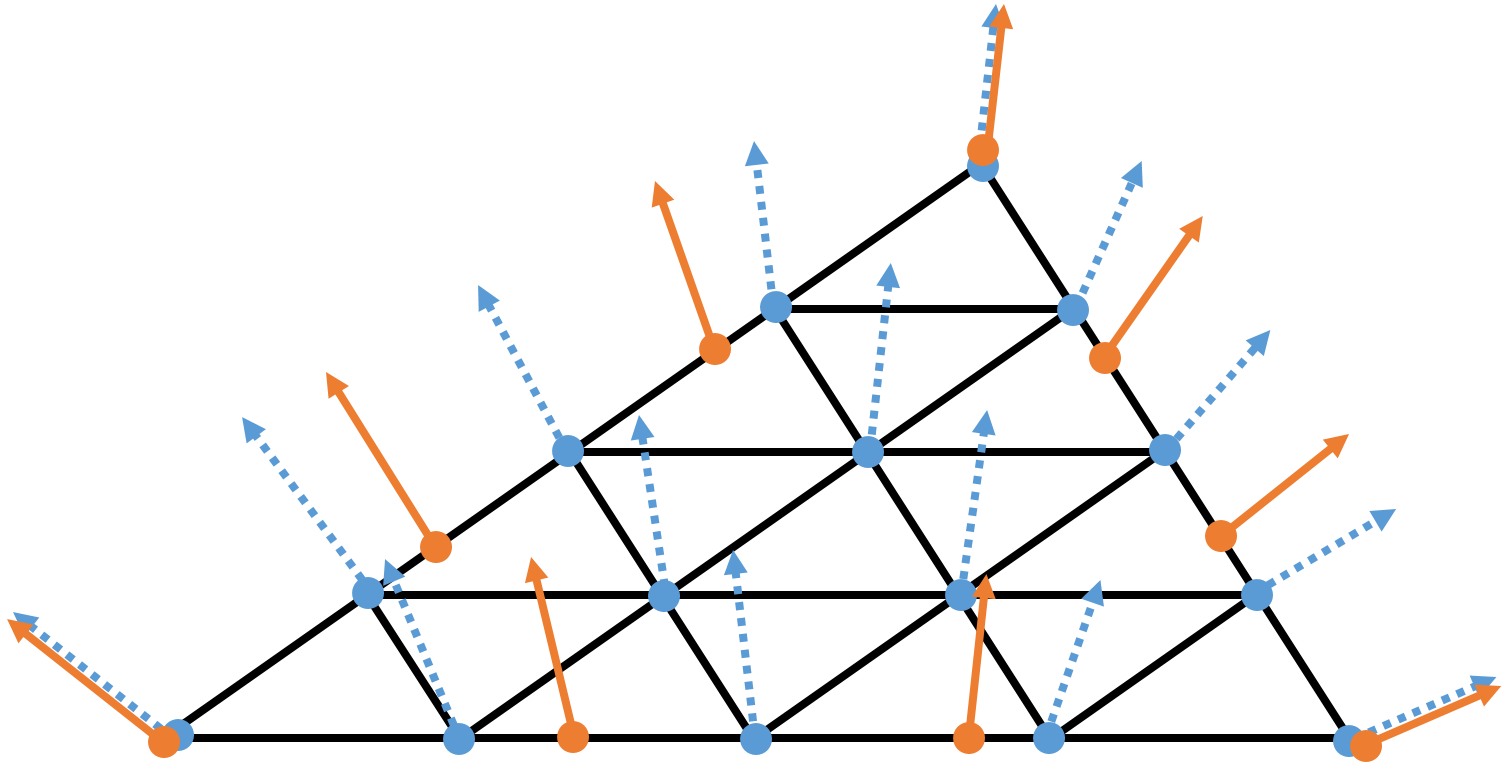
\includegraphics[width=\linewidth]{pic/normal_fitting_1.png}}
	\caption{Illustration of the fitting and constraint normals sampled on the triangle}
	\label{fig:normal_fitting}
%\end{figure}
\end{wrapfigure}

The above constrained normal field fitting can be formulated as follows. First, the $m$ fitting normals can be expressed as

\begin{equation}
	\footnotesize
		\left(
		\begin{array}{cccc}
		B^3_{300}(U_1) & B^3_{210}(U_1) & \cdots & B^3_{003}(U_1) \\
		B^3_{300}(U_2) & B^3_{210}(U_2) & \cdots & B^3_{003}(U_2) \\
		\vdots & \vdots & \ddots & \vdots \\
		B^3_{300}(U_m) & B^3_{210}(U_m) & \cdots & B^3_{003}(U_m) \\
		\end{array}
		\right)
		\left(
		\begin{array}{c}
		\mathbf P_0 \\
		\mathbf P_1 \\
		\vdots \\
		\mathbf P_9
		\end{array}
		\right)
		=
		\left(
		\begin{array}{c}
		\mathbf Q_1 \\
		\mathbf Q_2 \\
		\vdots \\
		\mathbf Q_m
		\end{array}
		\right)
	\label{equ:BPQ}
\end{equation}

\noindent where $\{U_k=(u_k,v_k,w_k)\}^m_{k=1}$ are the barycentric parameters of uniformly sampling normals ;
$\{\mathbf P_k\}_{k=0}^9$ are the control points of the cubic triangular B\'ezier patch for the normal field; and
$\{\mathbf Q_k\}_{k=1}^m$ are the deformed sampling normals corresponding to $\{U_k=(u_k,v_k,w_k)\}^m_{k=1}$.
Equation~\ref{equ:BPQ} can be rewritten as

\begin{equation}
	\footnotesize
	\mathbf M \mathbf P=\mathbf Q
\end{equation}

Then, the $3k(k=3)$ constraint normals can be expressed as:

\begin{equation}
	\footnotesize
		\left(
		\begin{array}{cccc}
		B^3_{300}(U_{s_1}) & B^3_{210}(U_{s_1}) & \cdots & B^3_{003}(U_{s_1}) \\
		B^3_{300}(U_{s_2}) & B^3_{210}(U_{s_2}) & \cdots & B^3_{003}(U_{s_2}) \\
		\vdots & \vdots & \ddots & \vdots \\
		B^3_{300}(U_{s_9}) & B^3_{210}(U_{s_9}) & \cdots & B^3_{003}(U_{s_9}) \\
		\end{array}
		\right)
		\left(
		\begin{array}{c}
		\mathbf P_0 \\
		\mathbf P_1 \\
		\vdots \\
		\mathbf P_9
		\end{array}
		\right)
		=
		\left(
		\begin{array}{c}
		\mathbf {\bar Q}_1 \\
		\mathbf {\bar Q}_2 \\
		\vdots \\
		\mathbf {\bar Q}_9
		\end{array}
		\right)
	\label{equ:BPQ_bar}
\end{equation}

\noindent where $\{U_{s_k}=(u_{s_k},v_{s_k},w_{s_k})\}_{k=1}^9$ are the barycentric parameters of the constraint normals,
which are uniformly distributed along the boundaries of the triangular domain, and $\{\mathbf{\bar Q_k}\}_{k=1}^9 $ are
the deformed constraint normals. Equation~\ref{equ:BPQ_bar} can be rewritten as

\begin{equation}
	\footnotesize
	\mathbf{\bar M} \mathbf P=\mathbf{\bar Q}
\end{equation}

The constraint normal fitting is to minimize $(\mathbf M \mathbf P - \mathbf Q)^{\mathrm T}(\mathbf M \mathbf P -
\mathbf Q)$ subject to the constraint $\mathbf{\bar M} \mathbf P=\mathbf{\bar Q}$. Using the method of Lagrange
multipliers, we obtain

\begin{equation}
	\footnotesize
	\left(
		\begin{array}{cc}
			\mathbf M^{\mathrm T}\mathbf M & \mathbf{\bar M}^{\mathrm T} \\
			\mathbf{\bar M} & \mathbf O
		\end{array}
	\right)
	\left(
		\begin{array}{c}
			\mathbf P\\
			\bm{\Lambda}
		\end{array}
	\right)
	=
	\left(
		\begin{array}{cc}
			\mathbf M^{\mathrm T}& \mathbf O\\
			\mathbf O &\mathbf I
		\end{array}
	\right)
	\left(
		\begin{array}{c}
			\mathbf Q\\
			\mathbf {\bar Q}
		\end{array}
	\right)
	\label{equ:lagrange}
\end{equation}

\noindent where $\bm{\Lambda}$ is the vector of 9 Lagrange multipliers, $\mathbf O$ is a zero matrix, and $\mathbf I$ is
an identity matrix.

All the triangular B\'ezier patches of the normal field are of degree 3. Thus, Equation~\ref{equ:lagrange} can be
combined for all normal patches as follows:

\begin{equation}
	\footnotesize
	\left(
		\begin{array}{cc}
			\mathbf M^{\mathrm T}\mathbf M & \mathbf{\bar M}^{\mathrm T} \\
			\mathbf{\bar M} & \mathbf O
		\end{array}
	\right)
	\left(
		\begin{array}{c}
			\mathbb P^N\\
			\mathbb{\Lambda}^N
		\end{array}
	\right)
	=
	\left(
		\begin{array}{cc}
			\mathbf M^{\mathrm T}& \mathbf O\\
			\mathbf O &\mathbf I
		\end{array}
	\right)
	\left(
		\begin{array}{c}
			\mathbb Q^N\\
			\mathbb {\bar Q}^N
		\end{array}
	\right)
	\label{equ:lagrange2}
\end{equation}

$\mathbb P^N$ is the control points of all cubic triangular B\'ezier surfaces of normal field, $\mathbb \Lambda^N$ is
all of the Lagrange multipliers, and $\mathbb Q^N$ and $\mathbb{\bar Q}^N$ are the sampled fitting normals and sampled
constraint normals on all of the normal patches, respectively. The analytical solution to Equation~\ref{equ:lagrange2}
is:

\begin{equation}
	\footnotesize
	\left(
		\begin{array}{c}
			\mathbb P^N\\
			\mathbb{\Lambda}^N
		\end{array}
	\right)
	=
	\left(
		\begin{array}{cc}
			\mathbf M^{\mathrm T}\mathbf M & \mathbf{\bar M}^{\mathrm T} \\
			\mathbf{\bar M} & \mathbf O
		\end{array}
	\right)^{-1}
	\left(
		\begin{array}{cc}
			\mathbf M^{\mathrm T}& \mathbf O\\
			\mathbf O &\mathbf I
		\end{array}
	\right)
	\left(
		\begin{array}{c}
			\mathbb Q^N\\
			\mathbb {\bar Q}^N
		\end{array}
	\right)
	\label{equ:lagrange_solution}
\end{equation}

Due to the fixed sampling parameters, the product of the first two matrices on the right of
Equation~\ref{equ:lagrange_solution} is independent of the specific model. Thus they can be pre-computed and loaded if
necessary. Furthermore, the last 9 rows of the matrix product are about the solutions of Lagrange multipliers and can be
ignored. As a result, the control points of all cubic normal patches can be denoted as:

\begin{equation}
	\footnotesize
	\mathbb P^N = \mathbf M_r
	\left(
		\begin{array}{c}
			\mathbb Q^N\\
			\mathbb {\bar Q}^N
		\end{array}
	\right)
	\label{equ:ctrl_points_solution_n}
\end{equation}

\noindent where $\mathbf M_r$ are the first 10 rows of
$$
	\footnotesize
	\left(
		\begin{array}{cc}
			\mathbf M^{\mathrm T}\mathbf M & \mathbf{\bar M}^{\mathrm T} \\
			\mathbf{\bar M} & \mathbf O
		\end{array}
	\right)^{-1}
	\left(
		\begin{array}{cc}
			\mathbf M^{\mathrm T}& \mathbf O\\
			\mathbf O &\mathbf I
		\end{array}
	\right)
$$

In this manner, we can obtain the continuous normal fields across the deformed model. Figure~\ref{fig:normal_refinement}
shows the shading result of Figure~\ref{fig:all_ffd:d}.

\begin{wrapfigure}{r}{0.29\textwidth}
	\centering
	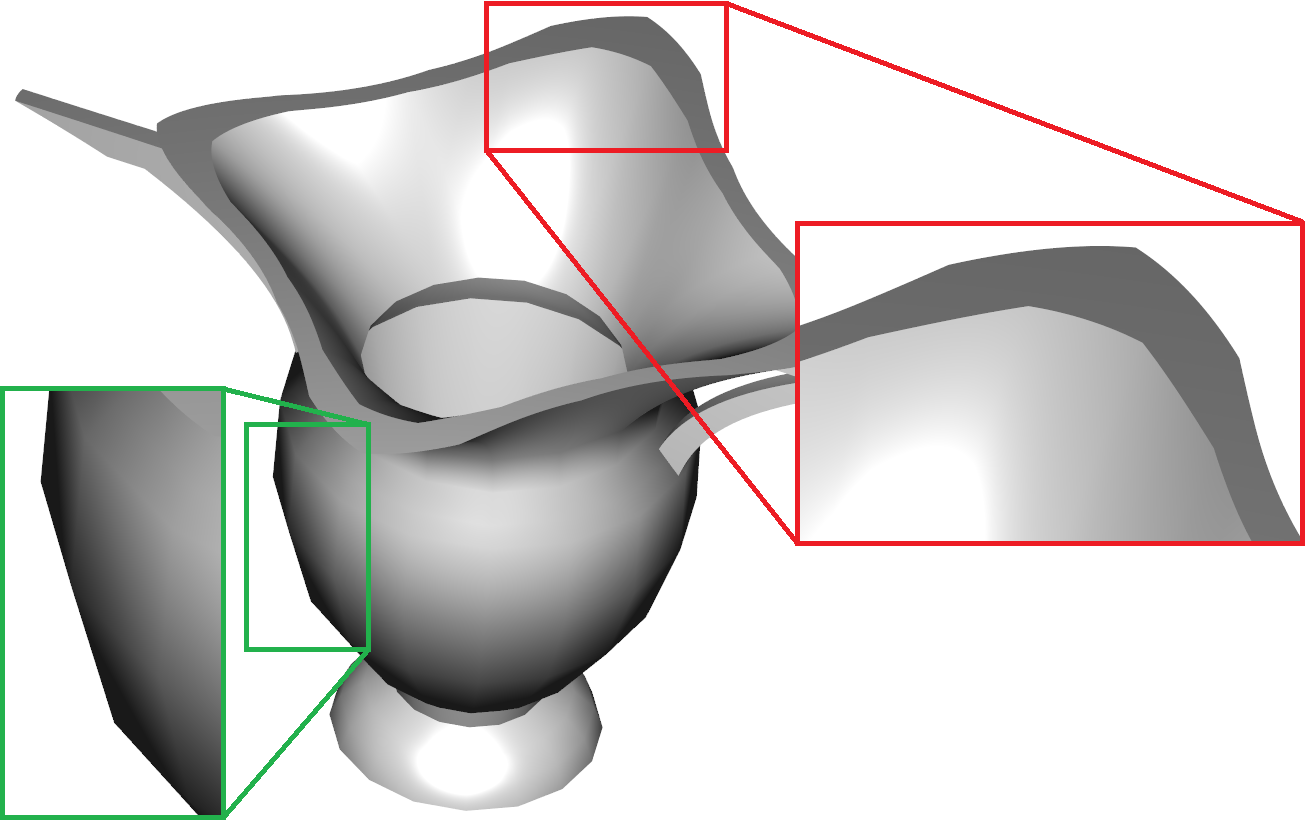
\includegraphics[width=\linewidth]{pic/normal_refinement_2.png}
	\caption{Shading result using constrained fitting normal field of the deformed model in Figure~\ref{fig:all_ffd:d}
	and its geometry artifacts.}
	\label{fig:normal_refinement}
\end{wrapfigure}

%%%%%%%%%%%%%

\subsection{Improvement of the deformed geometry}
\label{sec:geometry_fitting}

The shading in Figure~\ref{fig:normal_refinement} is smooth except for the geometry artifacts, i.e., the unsmooth
silhouettes and patch boundaries. Various solutions can be used to alleviate the artifacts for the Phong shading of
polygonal objects~\cite{Vlachos01, Boubekeur08}. A method inspired by the PN-triangles~\cite{Vlachos01} is proposed to
improve the silhouettes, patch boundaries, and keep the sharp edges.

In the PN-triangle algorithm~\cite{Vlachos01}, a cubic triangular B\'ezier patch is adopted to replace the corresponding
triangle to obtain a smooth geometry appearance in Phong shading. In the accurate FFD, the deformed object is
represented in terms of triangular B\'ezier patches~\cite{Feng98, Feng00, Cui14}, whose degree is the degree of the
B-spline volume, and is typically higher than 3. High degree will result in high computational costs. Furthermore, the
corresponding geometry adjustment becomes complex because there are many more control points. According to our
experiments, the cubic triangular B\'ezier patch is feasible and sufficiently flexible to approximate the geometry of
the accurate FFD result. Similar to the constrained normal field fitting approach in Section~\ref{sec:normal_fitting},
the geometry can be approximated by cubic triangular B\'ezier patches using the following equation:

\begin{equation}
	\footnotesize
	\mathbb P^V = \mathbf M_r
	\left(
		\begin{array}{c}
			\mathbb Q^V\\
			\mathbb {\bar Q}^V
		\end{array}
	\right)
	\label{equ:ctrl_points_solution_v}
\end{equation}

\noindent where $\mathbb P^V$ is the control points of all cubic triangular B\'ezier patches of the deformed object.
$\mathbb Q^V$ and $\mathbb {\bar Q}^V$ are those sampled fitting points and sampled constraint points on all cubic
triangular B\'ezier patches, respectively. The sampling strategy is the same as that of the normal field in
Section~\ref{sec:normal_fitting}.

Using the above method, a \textcolor{red}{$C^0$} continuous geometry and a
\textcolor{red}{$C^0$}/\textcolor{red}{discontinuous} normal field across the smooth and sharp edges are obtained. Next,
the geometry is adjusted to obtain a smooth geometry appearance along smooth edges and to preserve shape features along
sharp edges.

\begin{wrapfigure}{r}{0.3\textwidth}
		\centering
		\subfigure[Smooth edge]{\label{fig:sharp:a}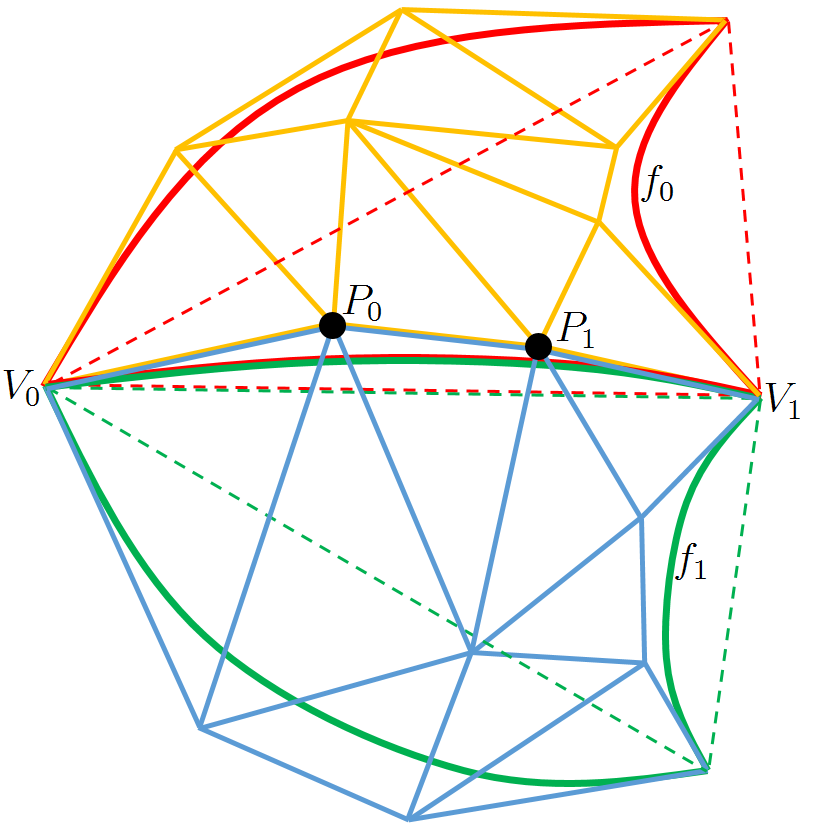
\includegraphics[width=0.47\linewidth]{pic/sharp1.png}}
		\subfigure[Sharp edge]{\label{fig:sharp:b}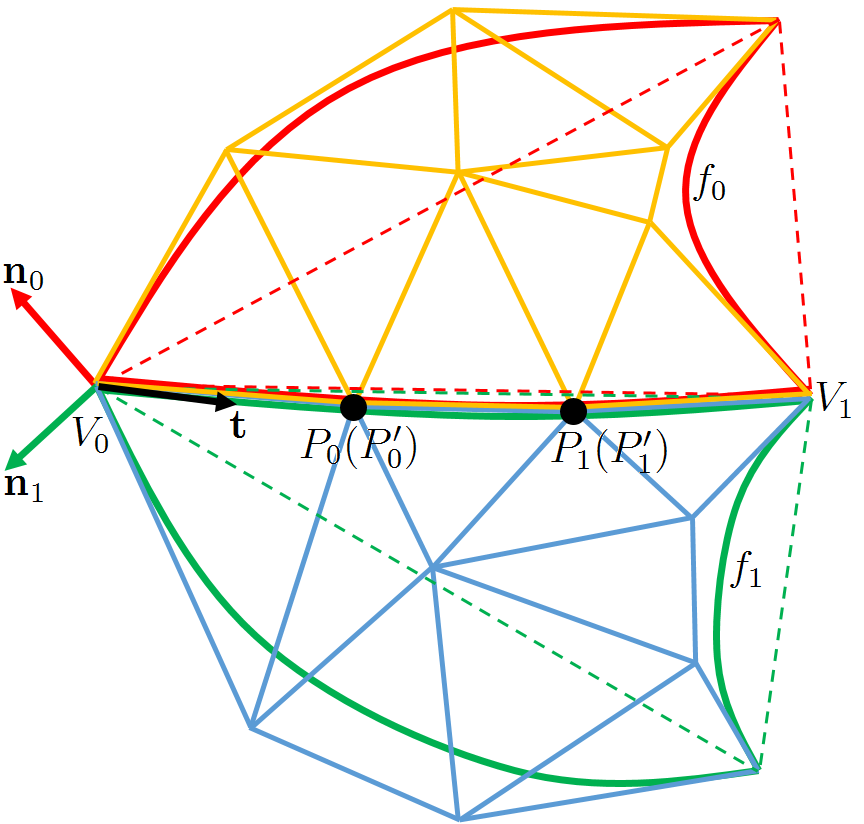
\includegraphics[width=0.50\linewidth]{pic/sharp3.png}}
		\caption{Adjustment of control points of the deformed geometry}
		\label{fig:sharp}
\end{wrapfigure}

The adjustment of triangular B\'ezier patches sharing a smooth edge is similar to the PN-triangle method. As shown in
Figure~\ref{fig:sharp:a}, the PN-triangle approach projects $(2V_0+V_1)/3$ into the tangent plane at $V_0$
\cite{Vlachos01}, whereas the proposed method projects the corresponding edge control point $P_0$ onto the tangent plane
at $V_0$. Thus, a visually plausible smooth geometry (\textcolor{red}{$C^0$} in fact) across the smooth edge is
obtained. In Figure~\ref{fig:sharp:a}, red and green dashed lines indicate two original triangles, and red and green
solid curve nets indicate cubic triangular B\'ezier patches, which are the adjustment results.

Similarly, the geometry adjustment of patches sharing a sharp edge is shown in Figure~\ref{fig:sharp:b}. The two
corresponding control points $P_0$ and $P_0'$ in the neighboring triangular B\'ezier patch $f_0$ and $f_1$ sharing a
sharp edge are projected to the vector $\mathbf t = \mathbf n_0 \times \mathbf n_1$, where $\mathbf n_0$ and $\mathbf
n_1$ are two distinct normals at the same vertex $V_0$. This method yields a \textcolor{red}{$C^0$} continuous geometry
across a sharp edge, which can preserve the sharp feature along the sharp edge.

After the above adjustment, visually plausible smooth geometries, such as silhouettes and edges, will be obtained. The
sharp features along the sharp edges are also preserved. An example is shown in Figure~\ref{fig:final_result}.
\textcolor{red}{It is worth noting that the generated geometry is different than the original discrete polygonal mesh
in the rest-pose because of the higher-order interpretation of the polygonal mesh.}


\begin{wrapfigure}{r}{0.2\textwidth}
	\centering
	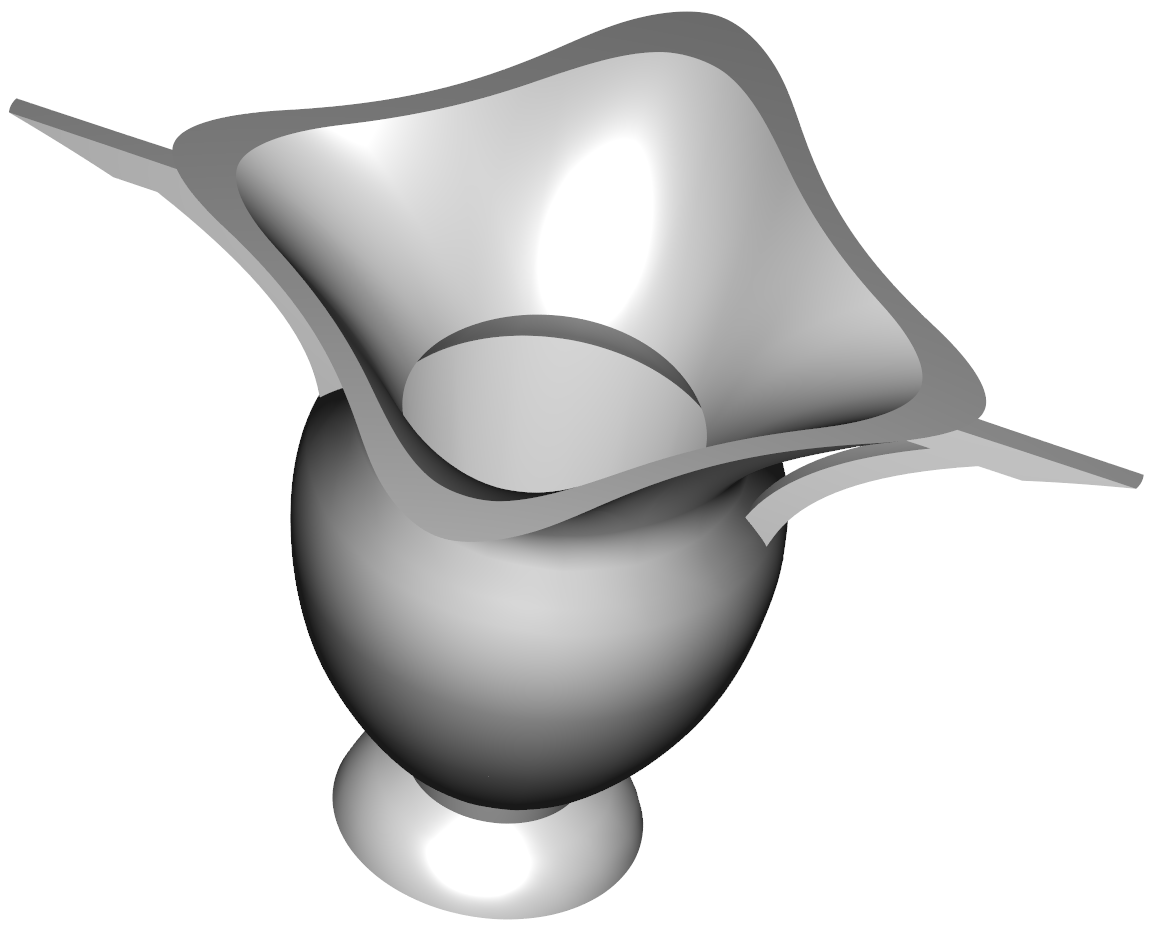
\includegraphics[width=1.0\linewidth]{pic/final_result.png}
	\caption{Shading result after adjusting the deformed geometry in Figure~\ref{fig:normal_refinement}}
	\label{fig:final_result}
\end{wrapfigure}

%%%%%%%%%%%%%%%

\subsection{Consideration of knot box clipping}

If there is only one knot box, the above deformed geometry and normal field methods are suitable. However, for the case
of general B-spline volumes, the input polygonal object will be clipped against the knot boxes, and thus, all of the
sub-triangles will lie in one knot box. If the above adjustment method is directly applied to the subdivided polygonal
object, the deformed geometry does not appear fair near the knots. An example is shown in Figure~\ref{fig:unfairness}.
Figure~\ref{fig:unfairness:a} is the deformed geometry by a B-spline volume with multiple knot boxes. Both the geometry
and shading are smooth. However, the geometry appearance is not fair. The \textcolor{red}{bold} curves are the deformed
curves corresponding to the original triangles on the model; the \textcolor{red}{thin} curves are the deformed curves of
the sub-triangles resulting from knot box clipping and subsequent triangulation. The unfair parts are indicated in the
red rectangles in Figure~\ref{fig:unfairness:b}. Since the sub-triangles from one original triangle are co-planar, the
constrained fittings for these deformed sub-triangles will lead to unfairness.

\begin{figure}[htbp]
\begin{center}
	\begin{minipage}[c]{0.62\textwidth}
		\centering
		\subfigure[Shading result with boundary curves]{\label{fig:unfairness:a}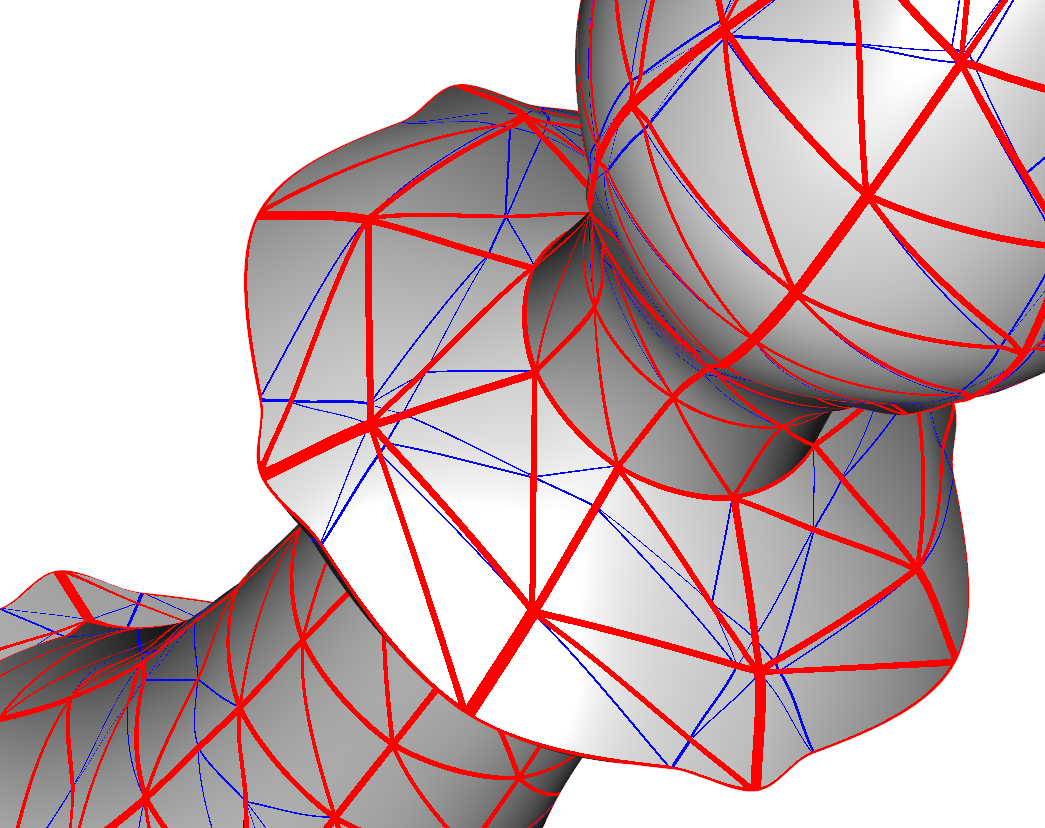
\includegraphics[width=0.32\linewidth]{pic/clipping2.png}}
		\subfigure[Shading result]{\label{fig:unfairness:b}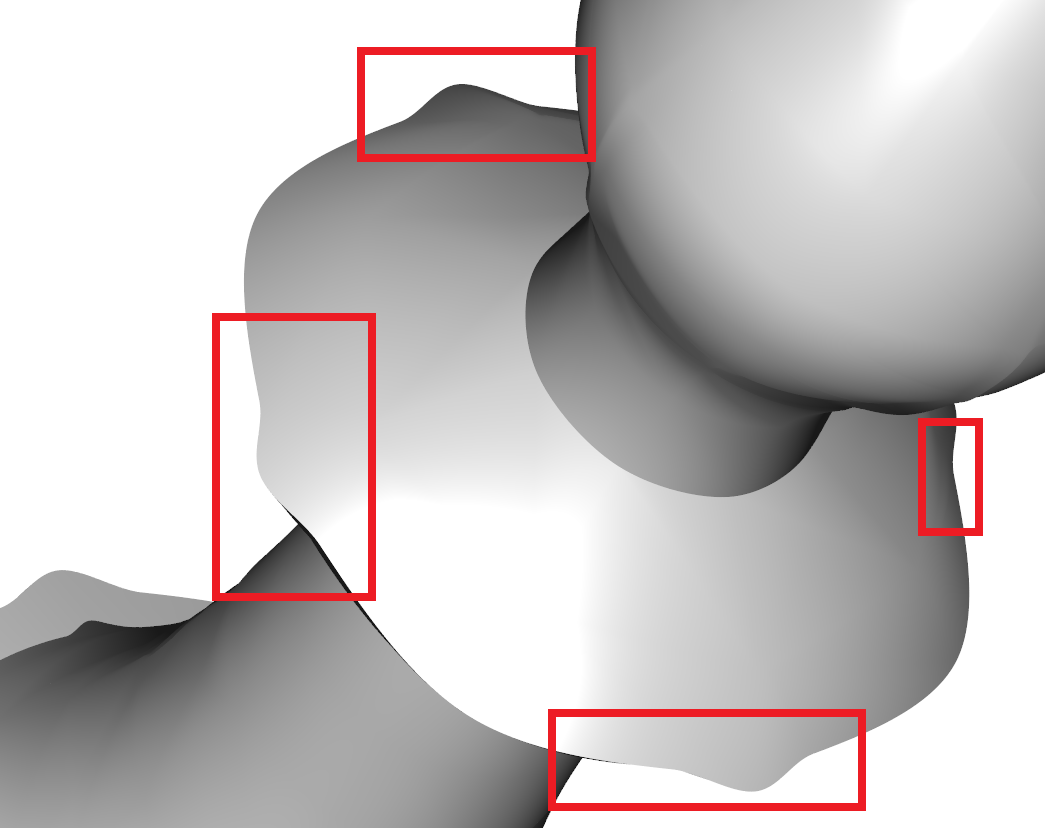
\includegraphics[width=0.32\linewidth]{pic/clipping1.png}}
		\subfigure[Visually plausible smooth and fair deformed geometry]{\label{fig:unfairness:c}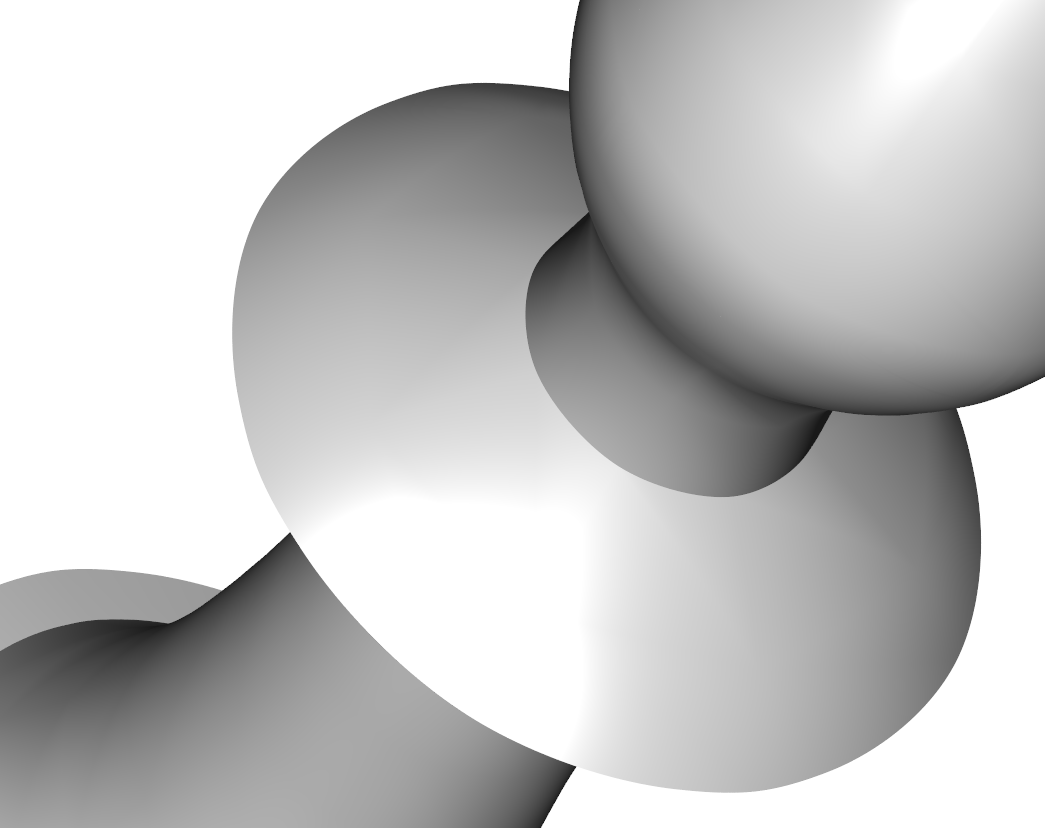
\includegraphics[width=0.32\linewidth]{pic/clipping3.png}}
		\caption{Unfairness near the clipping points in the deformed geometry and the improvement}
		\label{fig:unfairness}
	\end{minipage}
~
	\begin{minipage}[c]{0.36\textwidth}
		\centering
		\subfigure[Shading result with boundary curves]{\label{fig:linear_normal:a}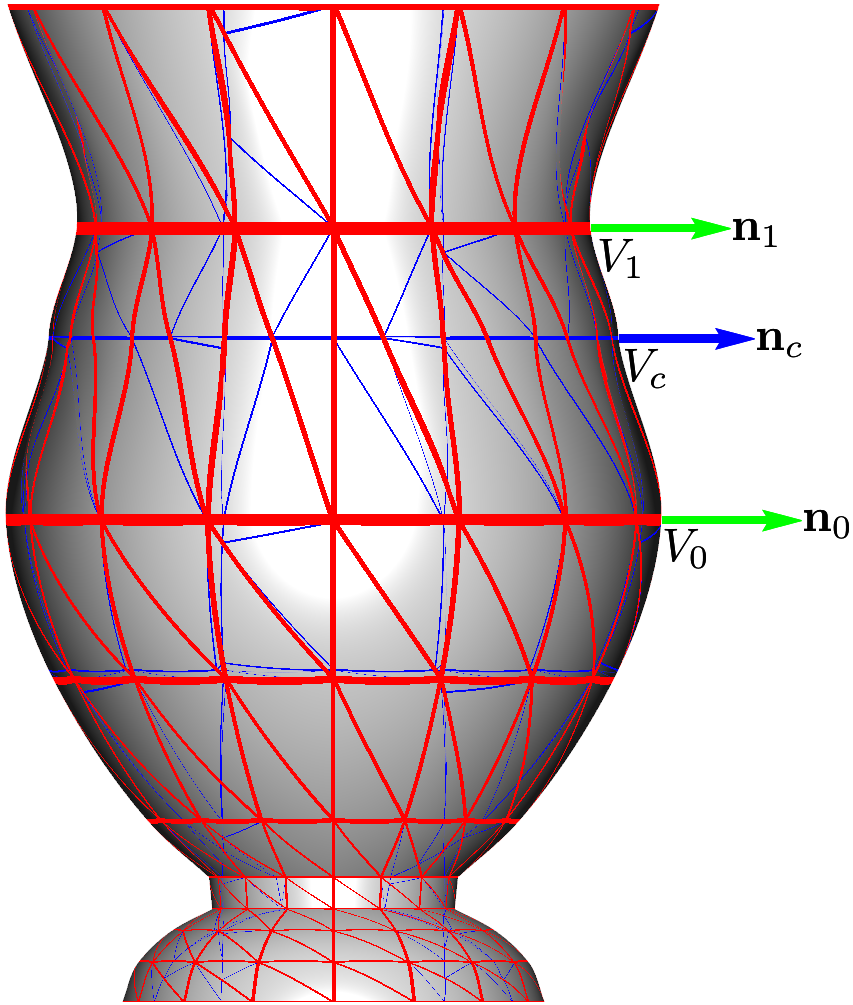
\includegraphics[width=0.37\linewidth]{pic/linear_normal_2.png}}
		\subfigure[Shading result]{\label{fig:linear_normal:b}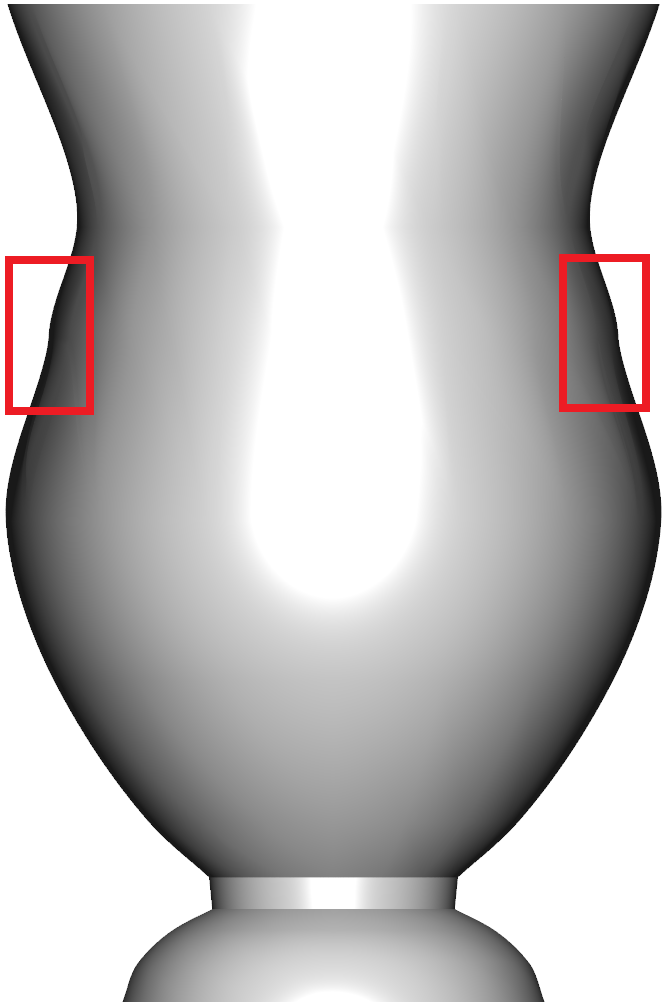
\includegraphics[width=0.29\linewidth]{pic/linear_normal_1.png}}
		\subfigure[Improved result of \ref{fig:linear_normal:a}]{\label{fig:linear_normal:c}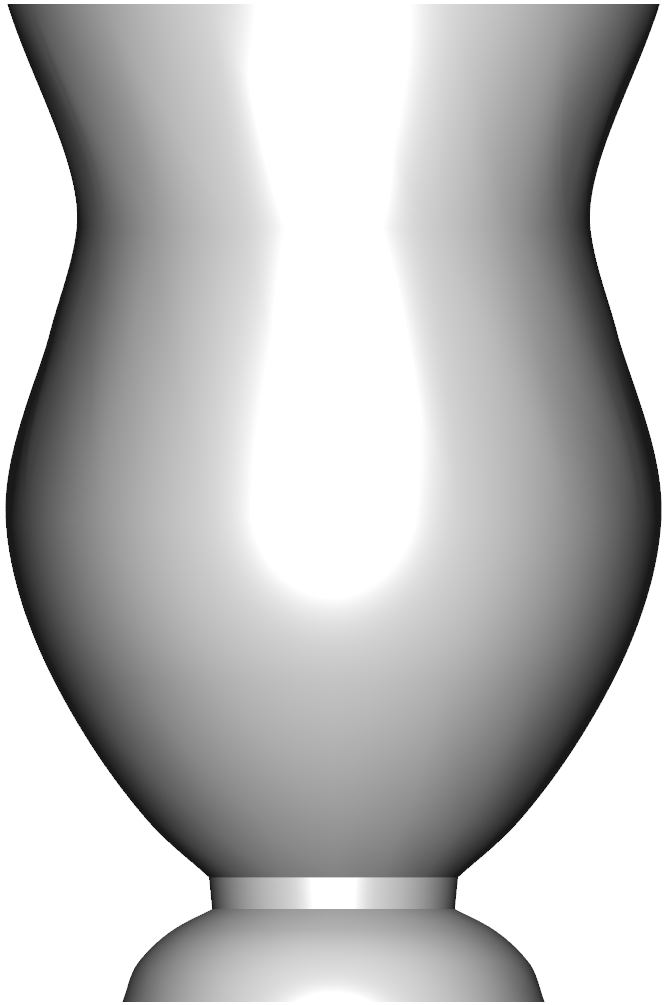
\includegraphics[width=0.29\linewidth]{pic/linear_normal_3.png}}
		\caption{The normal at the clipped vertex will lead to bumps and the related solution}
		\label{fig:linear_normal}
	\end{minipage}
\end{center}
\end{figure}

\subsubsection{Adjustment of the deformed geometry clipped against knot boxes}
\label{sec:clipped}

There is a heuristic solution to this unfairness problem. For each triangle in the original object, the corresponding
PN-triangle is generated first. If the triangle is subdivided against the knot boxes, the clipped vertices are moved to
the corresponding positions on the PN-triangle. Then, we apply the constrained fitting approach to the modified
sub-triangles. As a result, we can obtain a visually plausible smooth and fair deformed geometry. The improved result of
the example in Figure~\ref{fig:unfairness:a} is shown in Figure~\ref{fig:unfairness:c}.

\subsubsection{Normal adjustment at the clipped vertex}
\label{sec:normal_adjustment}

Intuitively, the normal at the clipped vertex can be calculated via barycentric coordinate interpolation. But it would
lead to an unfairness problem in the normal field as shown in Figure~\ref{fig:linear_normal:a} and
\ref{fig:linear_normal:b}. The normals of $V_0$ and $V_1$ are $\mathbf n_0$ and $\mathbf n_1$, respectively. Both of the
normals are horizontally rightward. Thus, the interpolated normal $\mathbf n_c$ of the subdivided vertex $V_c$ is also
horizontally rightward. There is no artifact when using the normal $\mathbf n_c$ to determine the normal field for
rendering. However, if it is used to adjust the control points for smoothing the deformed geometry, i.e., the edge
control points adjacent to $V_c$, it will lead to abnormal bumps on the deformed geometry.

The solution to this problem is to define a reasonable normal at each clipped vertex. The normal at the subdivided
vertex can take the corresponding normal $\mathbf n^*$ on the quadratic triangular B\'ezier normal field of the
PN-triangle~\cite{Vlachos01}. After using $\mathbf n^*$ in the geometry adjustment scheme, the adjusted geometry for the
example in Figure~\ref{fig:linear_normal:a} is shown in Figure~\ref{fig:linear_normal:c}, where the abnormal bumps
disappear. The adjusted normal field is only for smoothing the deformed geometry in Section~\ref{sec:geometry_fitting},
where some edge control points are projected onto the planes or tangent lines determined by the normals. The normal
field for rendering the deformed object is the normal field constructed in Section~\ref{sec:normal_fitting}, where the
normal at the clipped vertex is obtained via barycentric coordinate interpolation.

%%%%%%%%%%%%%%%%%%%%%%%%%%%%%%%%%%%%%%%%%%%%%%%%%%%%%%%%%%%%%%%%%%%%

\section{Parallel Implementation on the GPU}

The proposed algorithm contains a CPU execution component and a GPU execution component. As a data- and
computing-intensive algorithm, most of the computing overhead is implemented on the GPU. Because the algorithm is local,
it can fully utilize the parallel computing power of the GPU. The flowchart of the proposed algorithm is shown in
Figure~\ref{fig:workflow}. The \textcolor{red}{gray} boxes indicate the steps that are executed on the CPU. The
\textcolor{red}{white} boxes are the steps executed on the GPU and are the core of the proposed algorithm. NVIDIA CUDA
is used to perform the GPU computations.

\begin{figure}[htb]
	\centering
	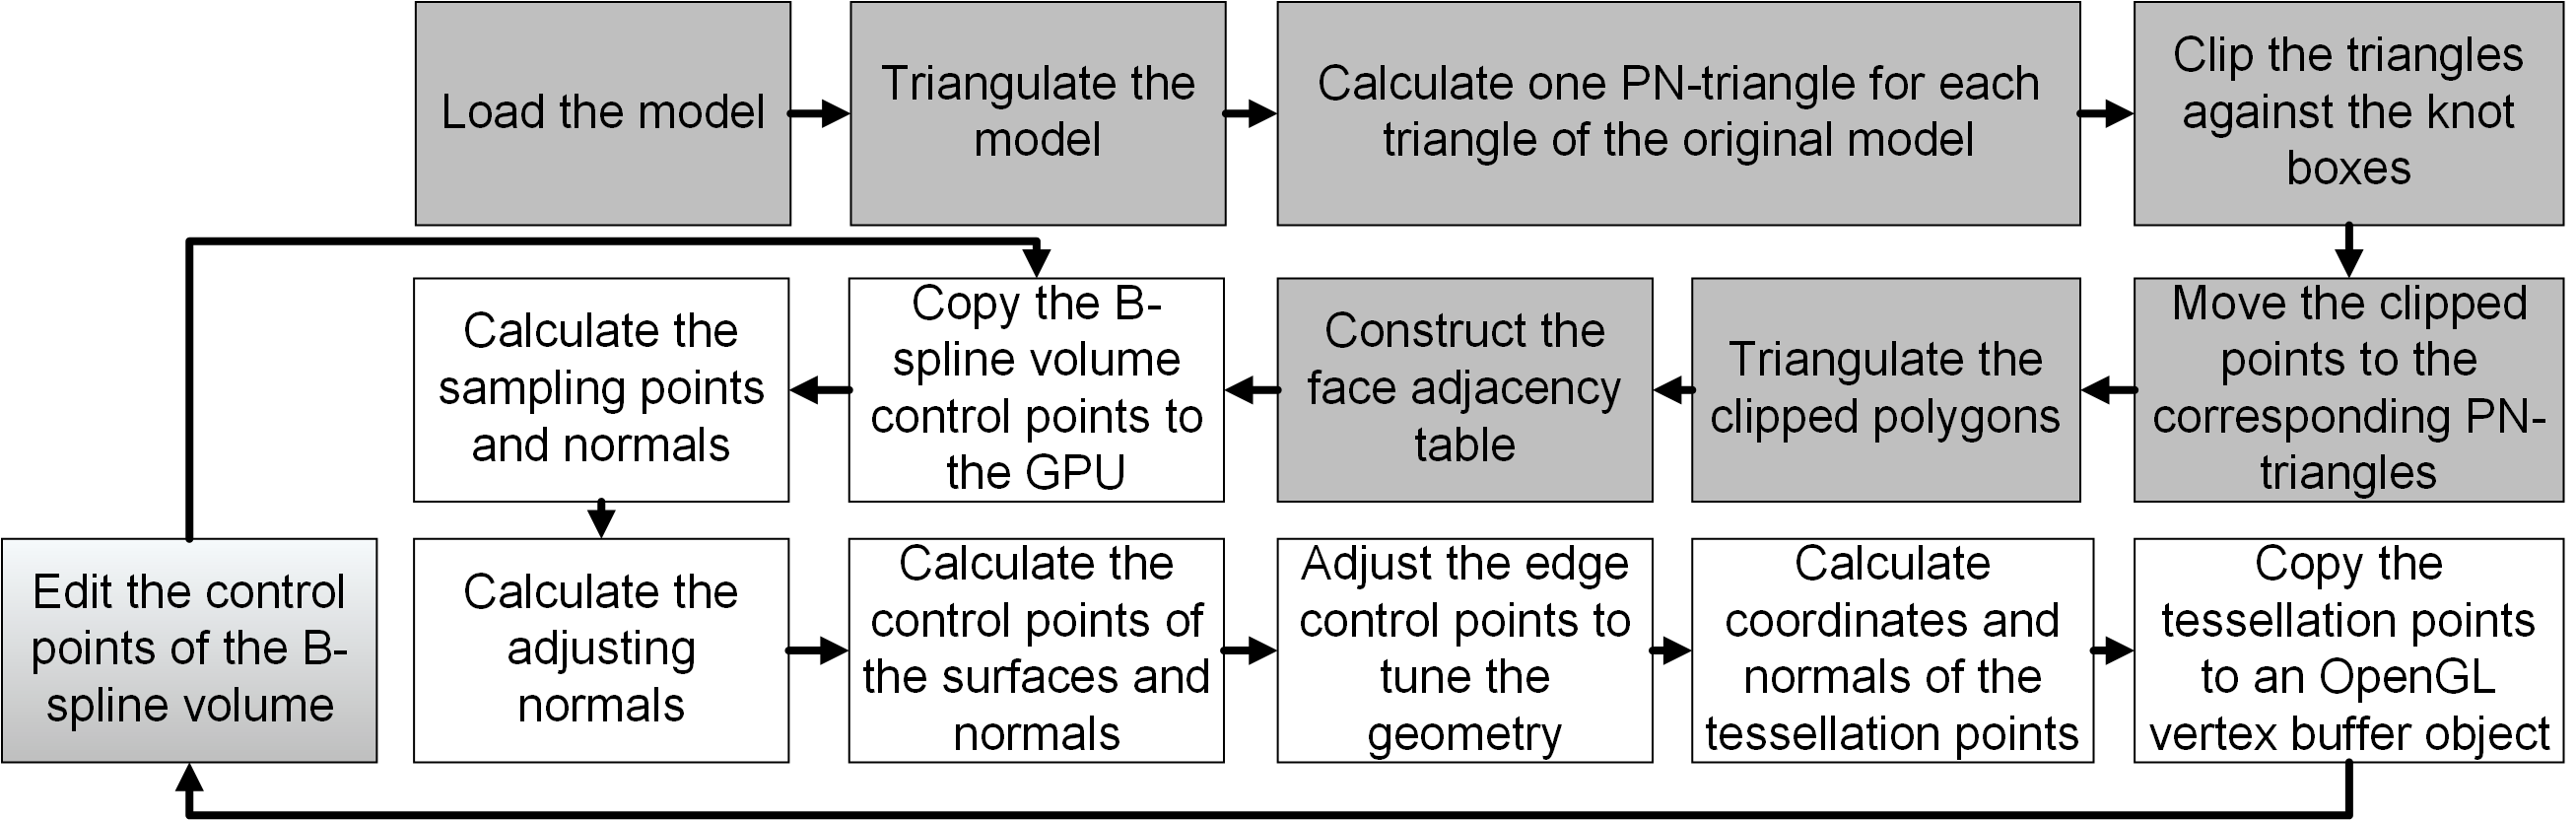
\includegraphics[width=0.8\linewidth]{pic/flowchart.png}
	\caption{Flowchart of the proposed algorithm}
	\label{fig:workflow}
\end{figure}

\subsection{Parallel computing sampling normals and points}

The first step in the proposed algorithm is to sample normals and points on the deformed object. More specifically, we
must calculate all elements in $\mathbb Q^N$ and $\mathbb {\bar Q}^N$ in Equation~\ref{equ:ctrl_points_solution_n} and
all elements in $\mathbb Q^V$ and $\mathbb {\bar Q}^V$ in Equation~\ref{equ:ctrl_points_solution_v}, which are the
control points of cubic triangular B\'ezier patches for the normal field and geometry, respectively.

$\mathbb Q^V$ and $\mathbb {\bar Q}^V$ can be directly obtained via B-spline volume evaluations. Two methods can be used
for this: the de Boor Cox algorithm and the matrix approach~\cite{Farin02}. We adopted the latter method because it is
less computationally burdensome and is more suitable for GPU implementation compared to the former method. The
deformation of a sampled normal in $\mathbb Q^N$ and $\mathbb {\bar Q}^N$ can be evaluated by
Equation~\ref{equ:gain_normal}.

In our implementation, one CUDA thread is used to calculate one sampling point and one sampling normal. Because each
cubic patch contains the same number of sampling points, the task arrangement is straightforward.

\subsection{Parallel computing constrained fitting patches for the geometry and normal field}

Having obtained $\mathbb Q^V$, $\mathbb {\bar Q}^V$, $\mathbb Q^N$ and $\mathbb {\bar Q}^N$, the next step is to
calculate the control points of the normal patches and geometry patches, i.e., the matrix $\mathbb P^N$ in
Equation~\ref{equ:ctrl_points_solution_n} and the matrix $\mathbb P^V$ in Equation~\ref{equ:ctrl_points_solution_v},
respectively. This can be accomplished by matrix multiplication. cuBLAS, which is a library of optimized implementations
of BLAS on a GPU, is adopted for these matrix multiplications \cite{cublas}. The elements of $\mathbb P^N$, $\mathbb
Q^N$, $\mathbb {\bar Q}^N$, $\mathbb P^V$, $\mathbb Q^V$ and $\mathbb {\bar Q}^V$ are 3-dimensional points, which are
not supported by cuBLAS. Thus, Equations~\ref{equ:ctrl_points_solution_n} and \ref{equ:ctrl_points_solution_v} should be
rewritten and combined as the following feasible form to fully explore the parallel computing power of the GPU:

\begin{equation}
	\footnotesize
	\left(
		\begin{array}{cccccc}
			\mathbb P^V_x & \mathbb P^V_y & \mathbb P^V_z & \mathbb P^N_x & \mathbb P^N_y & \mathbb P^N_z
		\end{array}
	\right)
	=
	\mathbf M_r
	\left(
		\begin{array}{cccccc}
			\mathbb Q^V_x & \mathbb Q^V_y & \mathbb Q^V_z & \mathbb Q^N_x & \mathbb Q^N_y & \mathbb Q^N_z\\
			\mathbb {\bar Q}^V_x & \mathbb {\bar Q}^V_y & \mathbb {\bar Q}^V_z & \mathbb {\bar Q}^N_x & \mathbb {\bar Q}^N_y & \mathbb {\bar Q}^N_z
		\end{array}
	\right)
	\label{equ:ctrl_points_solution_combine}
\end{equation}

\subsection{Calculating the adjusted normals for the subdivided geometry}

As described in Section~\ref{sec:normal_adjustment}, each sub-triangle has three adjustment normals, one for each
vertex. These vertex normals are taken from the corresponding points on the normal field of the PN-triangle of the
original triangle. Then, they undergo deformation via Equation~\ref{equ:gain_normal} for the silhouette adjustment. Here
we use one CUDA thread to handle one normal computation.

\subsection{Adjusting the edge control points in parallel on the GPU}

The main task in this step is finding 1-ring neighbors of the current triangle. A face adjacency table can accomplish
this task. The topological connectivity of the model remains unchanged during the deformation. Thus, the face adjacency
table can be constructed once in the pre-processing step and copied from the main memory to the GPU memory. The face
adjacency table is maintained in GPU via a hash table.

The topological connectivity of the model will be modified after the subdivision against the knot boxes (Step 4 in
Figure~\ref{fig:workflow}) and the triangulation of sub-polygons (Step 6 in Figure~\ref{fig:workflow}). Thus, the face
adjacency table must be reconstructed after subdivision and triangulation (Step 7 in Figure~\ref{fig:workflow}), copied
to the GPU memory, and used by the CUDA kernel.

After obtaining the adjusted normals, control points of the geometry patches, and the face adjacency table, we can
adjust the edge control points to tone the geometry using the method in Section~\ref{sec:geometry_fitting} in parallel.
Here, one CUDA thread is used to adjust one patch.

\subsection{GPU tessellations of the geometry and normal surfaces}

The triangular B\'ezier patches for the geometry and normal field have now been obtained. However, current GPUs do not
support the rendering of triangular B\'ezier patches directly. Thus, we must tessellate the patches into triangles for
rendering. Here, we use a uniform tessellation method in \cite{Cui14} to calculate the tessellated points and normals to
fully explore the tremendous computing power of the GPU. Similar to \cite{Cui14}, we combine the point and normal
evaluations as in Equation~\ref{equ:ctrl_points_solution_combine} for efficiency:

\begin{equation}
	\footnotesize
	\left(
		\begin{array}{cccccc}
			\mathbb R^V_x & \mathbb R^V_y & \mathbb R^V_z & \mathbb R^N_x & \mathbb R^N_y & \mathbb R^N_z
		\end{array}
	\right)
	=
	\mathbf B_q
	\left(
		\begin{array}{cccccc}
			\mathbb P^V_x & \mathbb P^V_y & \mathbb P^V_z & \mathbb P^N_x & \mathbb P^N_y & \mathbb P^N_z
		\end{array}
	\right)
	\label{equ:last}
\end{equation}

\noindent where $\mathbf B_q$ is the evaluation matrix of cubic triangular B\'ezier patches. The result can be rendered
using an OpenGL Vertex Buffer Object (VBO).

%%%%%%%%%%%%%%%%%%%%%%%%%%%%%%%%%%%%%%%%%%%%%%%%%%%%%%%%%%%%%%%%%%%%

\section{Implementation Results and Comparison}

The proposed method is implemented on a PC with an Intel Core i5 760 CPU@2.8GHz, 4 GB of main memory and an NVIDIA
GeForce GTX 465 GPU. The operating system is Arch Linux x86\_64. The CPU and GPU components of our method are written
using C++ and CUDA, respectively.

We will compare the proposed smooth FFD with a uniform upsampling method and \cite{Cui13, Cui14} from the aspects of
rendering result, efficiency and approximation errors, tessellation in the follows.

\subsection{Comparison of the rendering results}
\label{sec:comparison_of_rendering}

The deformation results are shown in Figure~\ref{fig:ship}-\ref{fig:rabbit}. Each triangular B\'ezier patch is
tessellated into 100 triangles. There are 4 sub-figures in each of the 4 examples: (a) is the original model; (b) is the
result of accurate FFD \cite{Cui13, Cui14}; (c) is the result of smooth FFD; (d) is the textured shading effect of (c).

\begin{figure}[htbp]
\begin{center}
	\begin{minipage}[l]{0.54\textwidth}
		\centering
		\subfigure[]{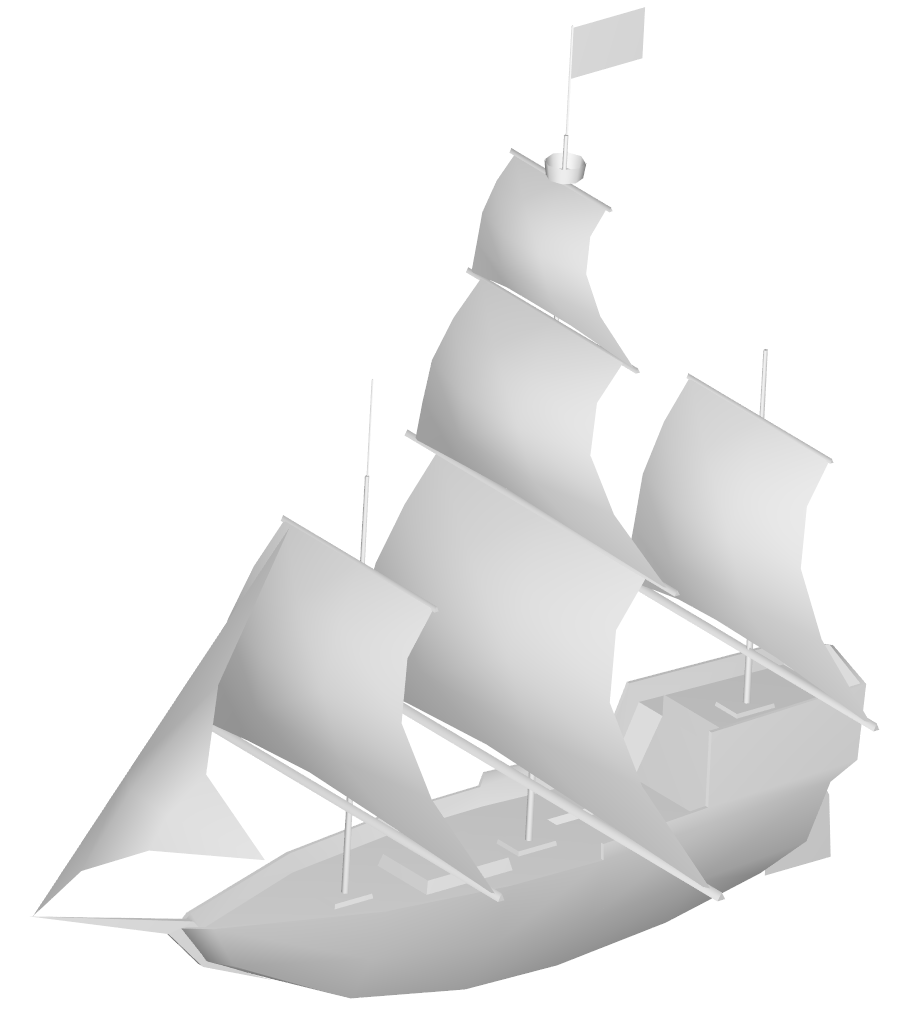
\includegraphics[width=0.24\linewidth]{pic/ship0.png}}
		\subfigure[]{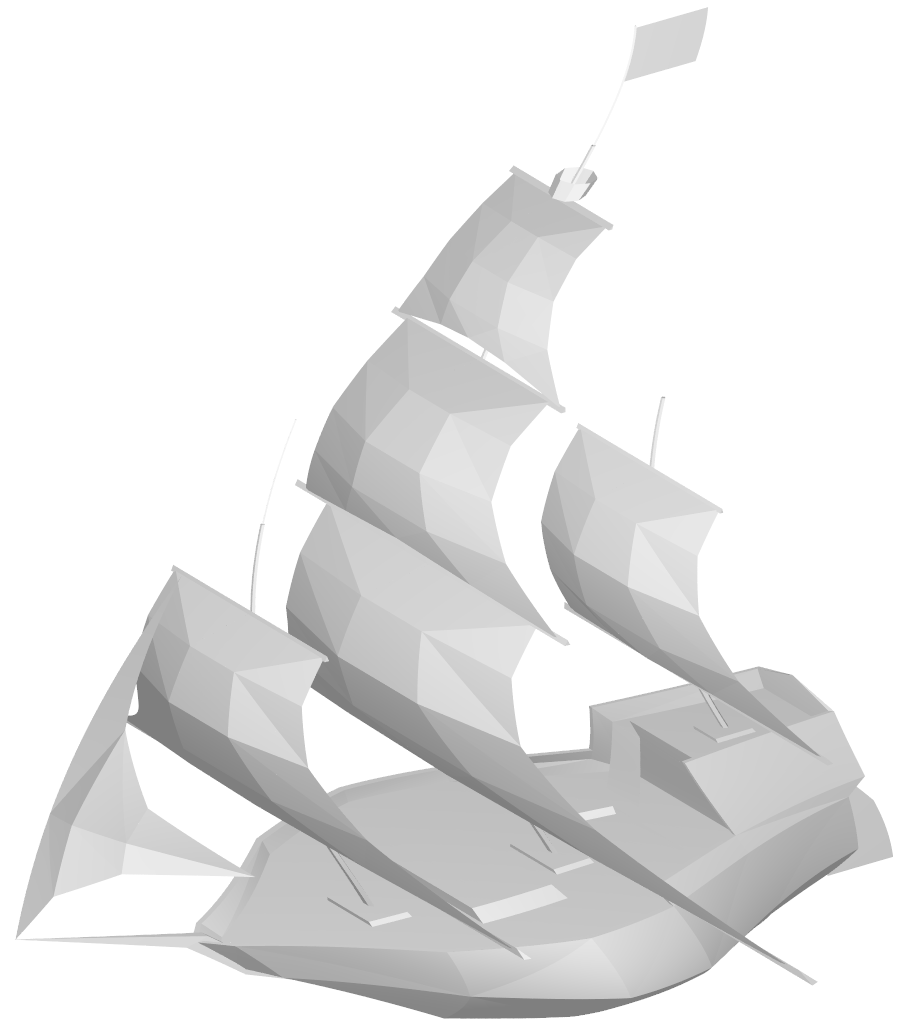
\includegraphics[width=0.24\linewidth]{pic/ship1.png}}
		\subfigure[]{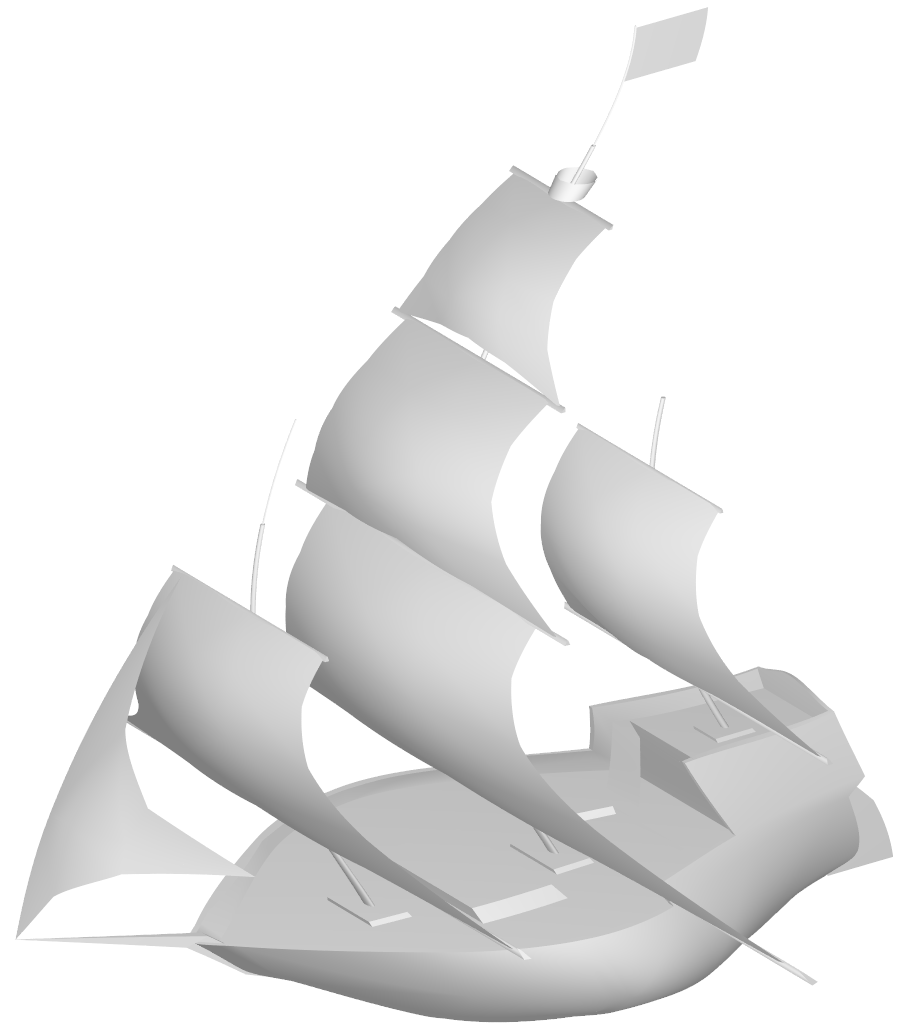
\includegraphics[width=0.24\linewidth]{pic/ship2.png}}
		\subfigure[]{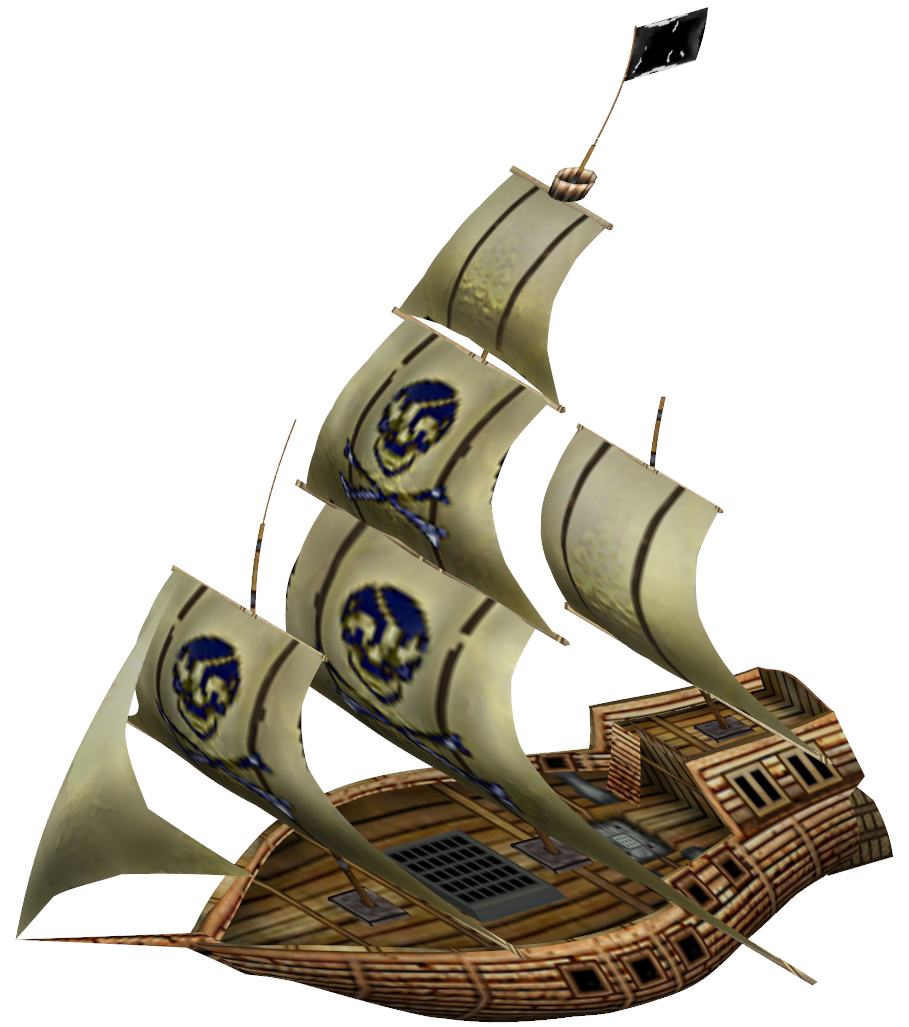
\includegraphics[width=0.24\linewidth]{pic/ship3.png}}
		\caption{Deformation of the Ship model by a $3\times3\times3$ B-spline volume with $5\times8\times5$ control points}
		\label{fig:ship}
	\end{minipage}
~
	\begin{minipage}[r]{0.44\textwidth}
		\centering
		\subfigure[]{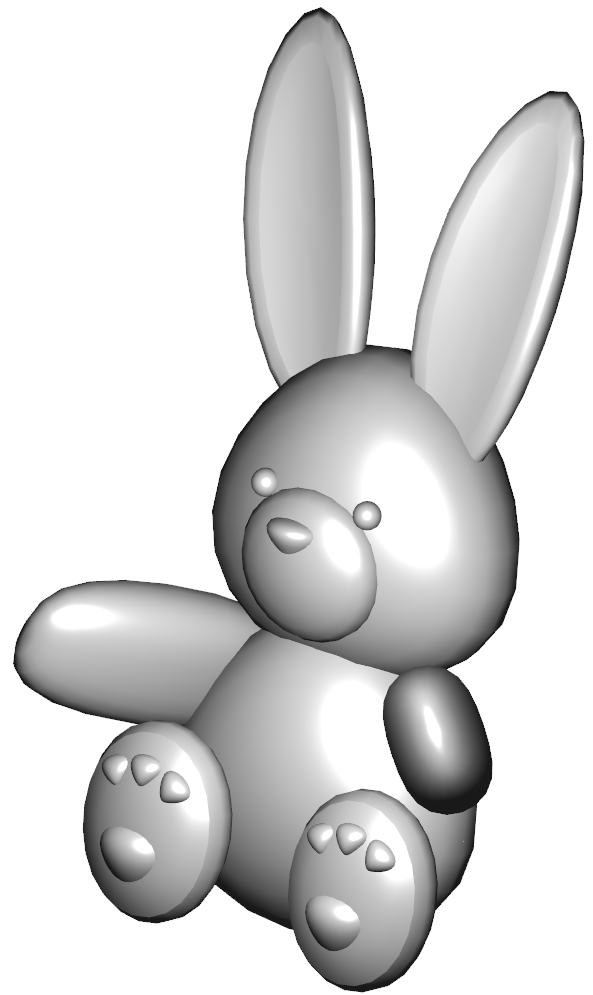
\includegraphics[width=0.2\linewidth]{pic/doll0.png}}
		\subfigure[]{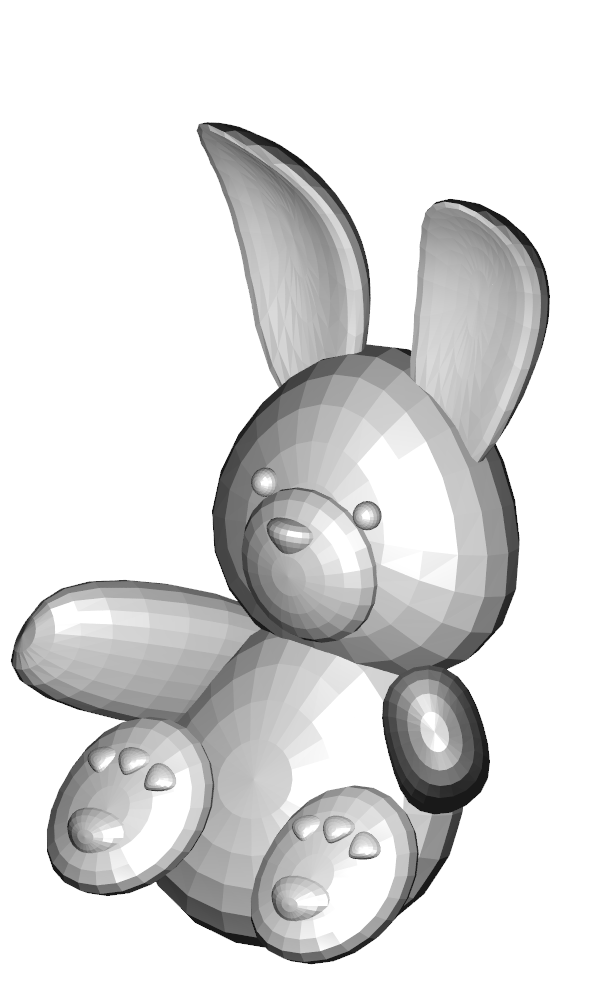
\includegraphics[width=0.2\linewidth]{pic/doll1.png}}
		\subfigure[]{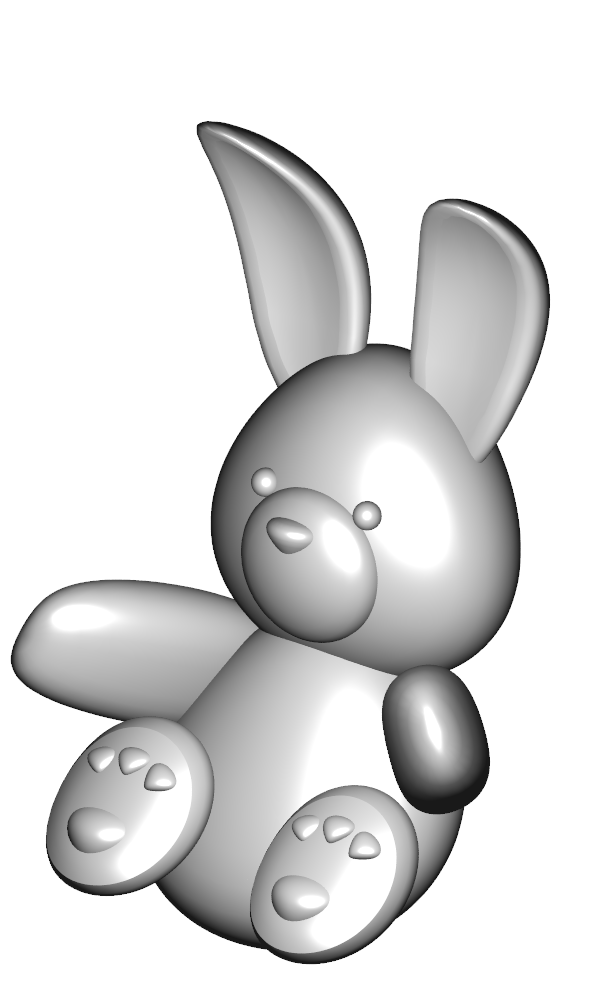
\includegraphics[width=0.2\linewidth]{pic/doll2.png}}
		\subfigure[]{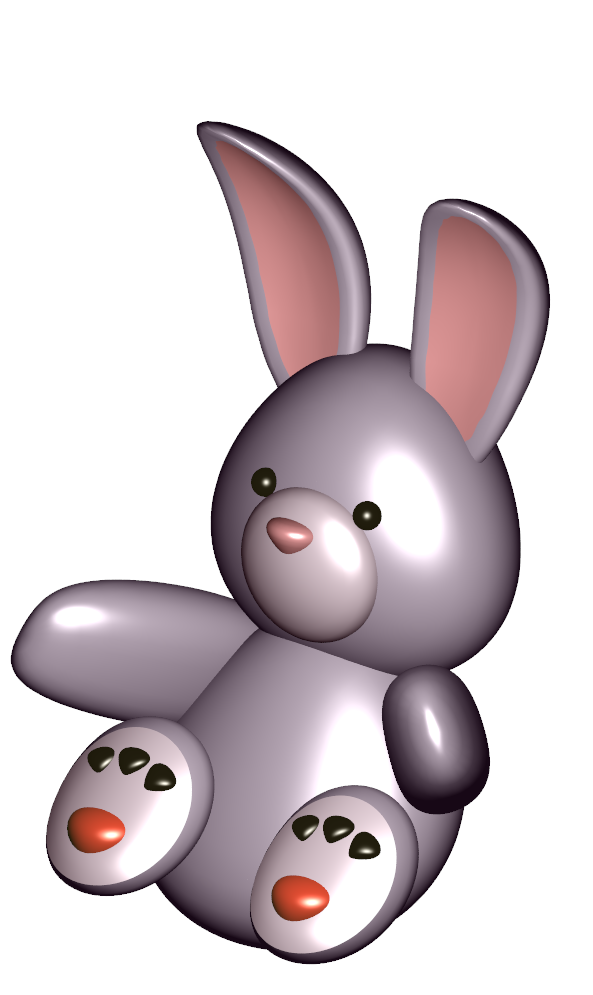
\includegraphics[width=0.2\linewidth]{pic/doll3.png}}
		\caption{Deformation of the Doll model by a $2\times2\times2$ B-spline volume with $5\times5\times5$ control points}
		\label{fig:doll}
	\end{minipage}
\end{center}
\end{figure}


\begin{figure}[htbp]
\begin{center}
	\begin{minipage}[c]{0.63\textwidth}
		\centering
		\subfigure[]{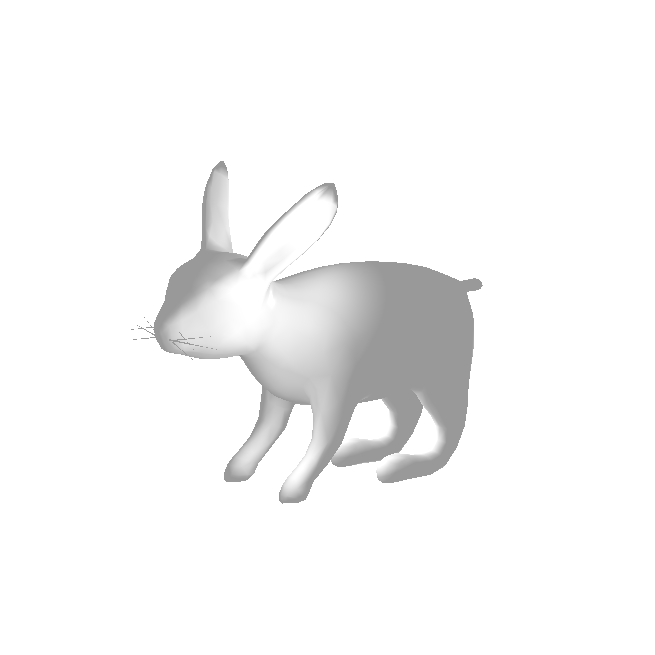
\includegraphics[width=0.242\linewidth]{pic/rabbit0.png}}
		\subfigure[]{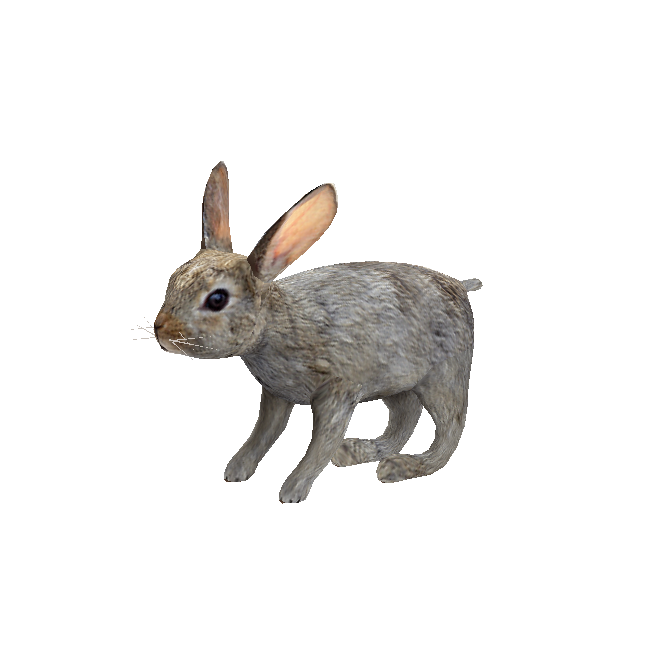
\includegraphics[width=0.242\linewidth]{pic/rabbit1.png}}
		\subfigure[]{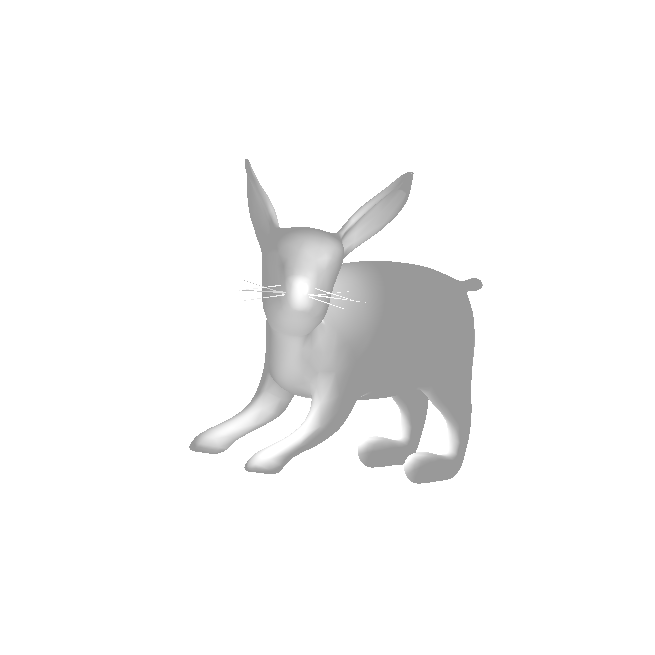
\includegraphics[width=0.242\linewidth]{pic/rabbit2.png}}
		\subfigure[]{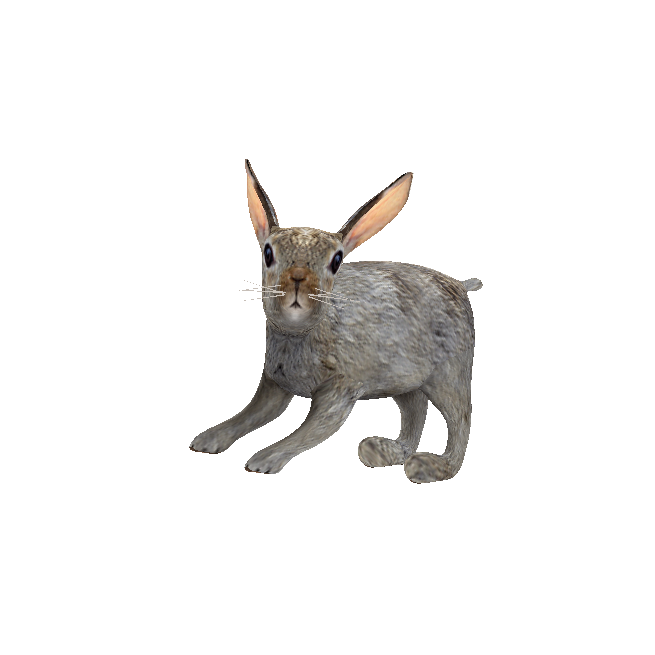
\includegraphics[width=0.242\linewidth]{pic/rabbit3.png}}
		\caption{Deformation of the Rabbit model by a $2\times2\times2$ B-spline volume with $5\times8\times5$ control points}
		\label{fig:rabbit}
	\end{minipage}
~
	\begin{minipage}[r]{0.35\textwidth}
		\centering
		\subfigure[]{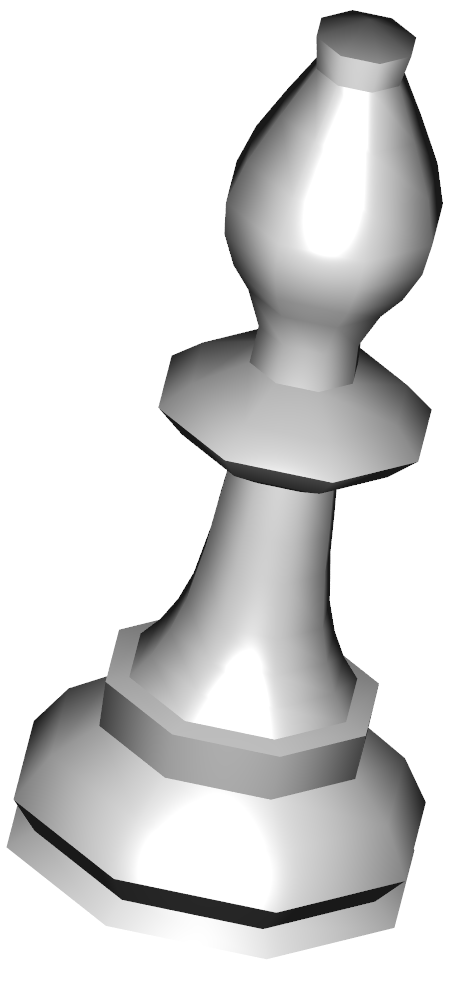
\includegraphics[width=0.189\linewidth]{pic/chess0.png}}
		\subfigure[]{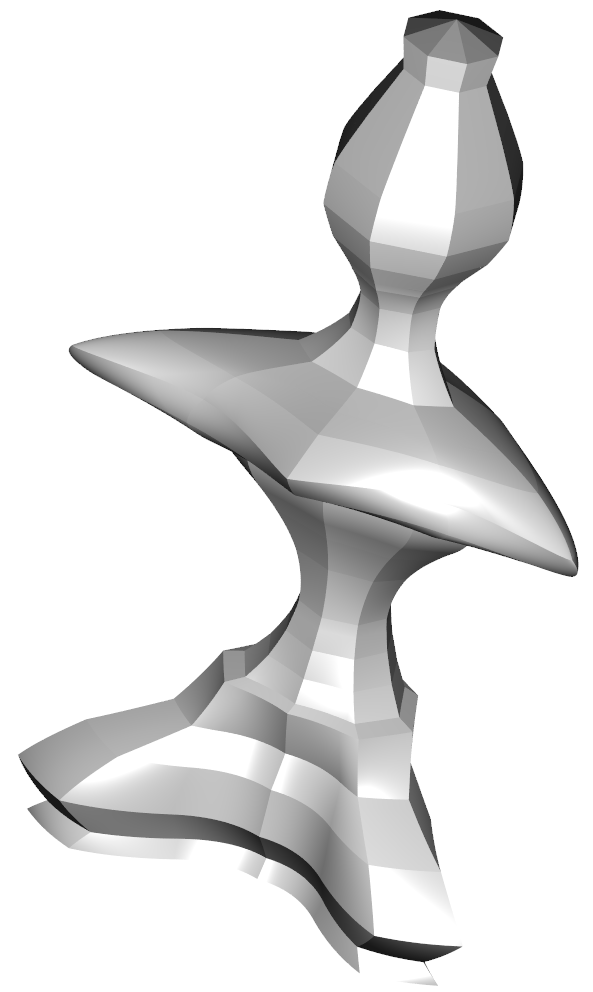
\includegraphics[width=0.245\linewidth]{pic/chess1.png}}
		\subfigure[]{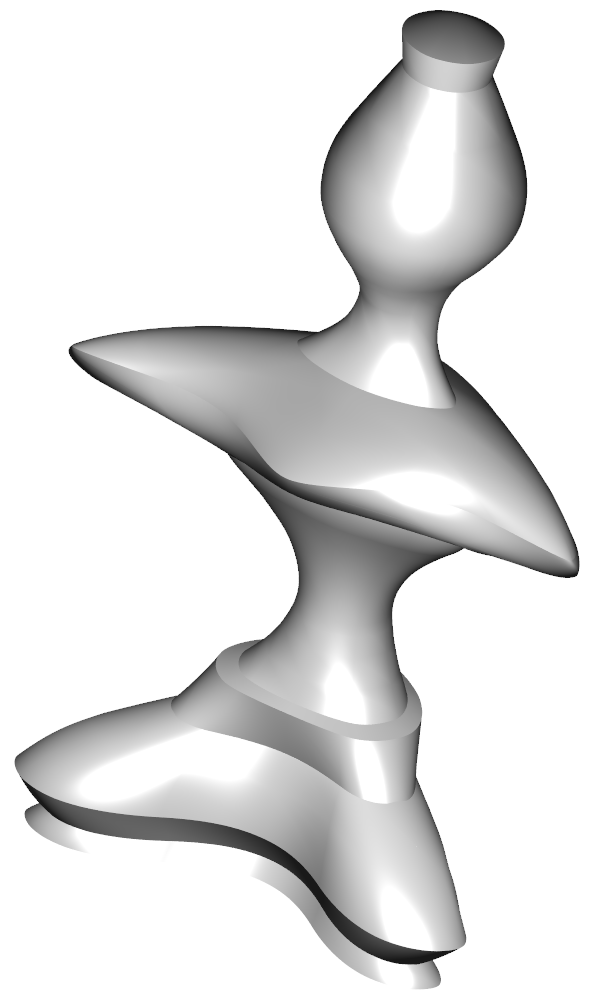
\includegraphics[width=0.245\linewidth]{pic/chess2.png}}
		\subfigure[]{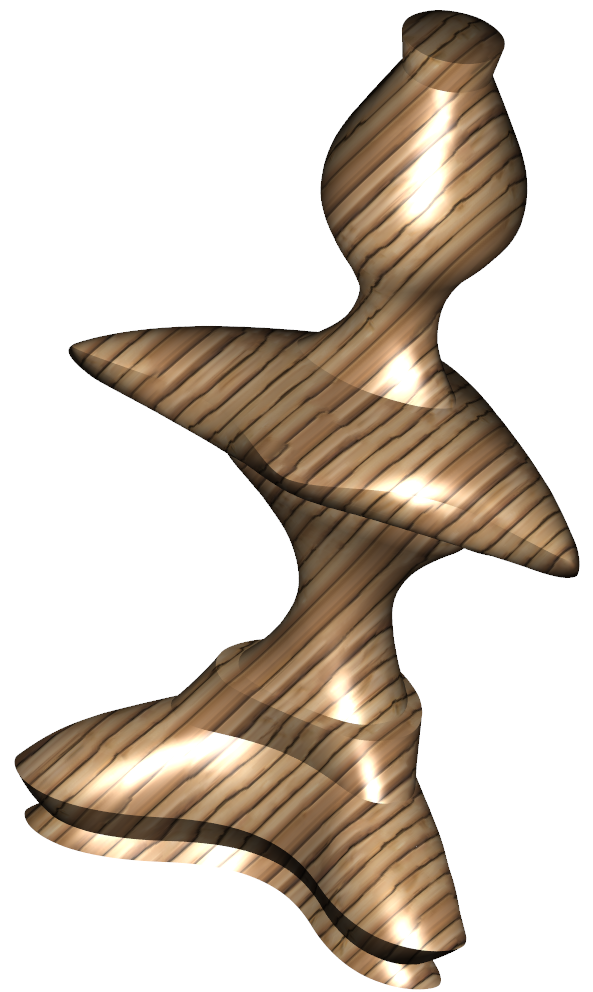
\includegraphics[width=0.245\linewidth]{pic/chess3.png}}
		\caption{Deformation of the Chess model by a $2\times2\times2$ B-spline volume with $5\times9\times5$ control points}
		\label{fig:chess}
	\end{minipage}
\end{center}
\end{figure}

These figures illustrate that the results obtained with smooth FFD are superior to those obtained with the other
methods. The highlight is smooth because the normals that we use are independent of the model geometry. The smooth
geometry and sharp features benefit from our geometry and normal adjustment method.

\subsection{Comparison of efficiencies}

The efficiencies obtained with smooth FFD and \cite{Cui13, Cui14} are compared in Table~\ref{tab:compare}. The model we
use is shown in Figure~\ref{fig:snail:a}; this model has 46,742 faces. As in Section~\ref{sec:comparison_of_rendering},
each triangular B\'ezier patch is tessellated into 100 sub-triangles. The degree of the B-spline volume is
$2\times2\times2$, with $5\times5\times5$ control points. Table~\ref{tab:compare} illustrates that the speed of our
method is lower than that of \cite{Cui14} due to additional geometry adjustment, normal field computation and
adjustment, but higher than that of \cite{Cui13}. The proposed method is sufficiently fast to handle large models in
real time.

\begin{figure}[htb] 
  \begin{minipage}[c]{0.29\textwidth} 
		\centering
		\subfigure[Shading of smooth FFD]{\label{fig:snail:a}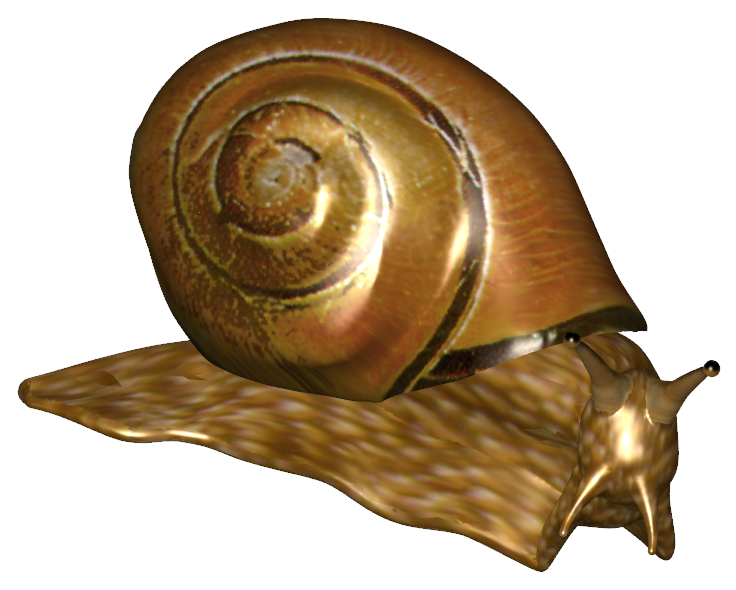
\includegraphics[width=0.46\linewidth]{pic/snail1.png}}
		\subfigure[Shading of UUS algorithm]{\label{fig:snail:b}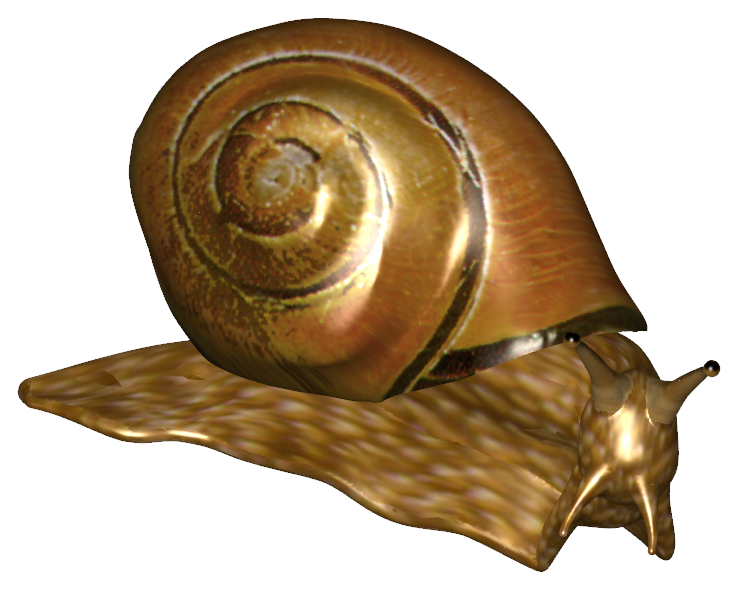
\includegraphics[width=0.46\linewidth]{pic/snail2.png}}
		\caption{Shading results for smooth FFD and UUS algorithm}
		\label{fig:snail}
  \end{minipage}
  \begin{minipage}[c]{0.7\textwidth} 
	\centering
	\footnotesize
	\tabcaption{Comparison of the efficiencies of our method, \cite{Cui13} and \cite{Cui14} (ms)}
	\begin{tabular}{llll}
		\hline
		Step & Our method & \cite{Cui13} & \cite{Cui14}\\
		\hline
		Copy control points to the GPU & 0.009 & 0.009 & 0.009 \\
		Calculate the sampling points & 8.469 & - & 6.701 \\
		Calculate the constraint points & 2.879 & - & - \\
		Calculate the control points & 3.971 & 11.608 & - \\
		Calculate the adjusting normals & 1.162 & - & - \\
		Adjust the control points & 2.003 & - & - \\
		Calculate the tessellation points & 4.861 & 24.33 & 7.507 \\
		Copy the results to the VBO & 3.092 & - & 3.301 \\
		render & 10.816 & 10.709 & 10.773 \\
		total & 37.262 & 46.656 & 28.291 \\
		\hline
	\end{tabular}
	\label{tab:compare}
  \end{minipage} 
\end{figure}

\subsection{Approximation error tests}

%\begin{wrapfigure}{r}{0.31\textwidth}
\begin{wrapfigure}{r}{0.35\textwidth}
%\begin{figure}[htbp]
\begin{center}
	\centering
	\subfigure[\textcolor{red}{Original model}]{
		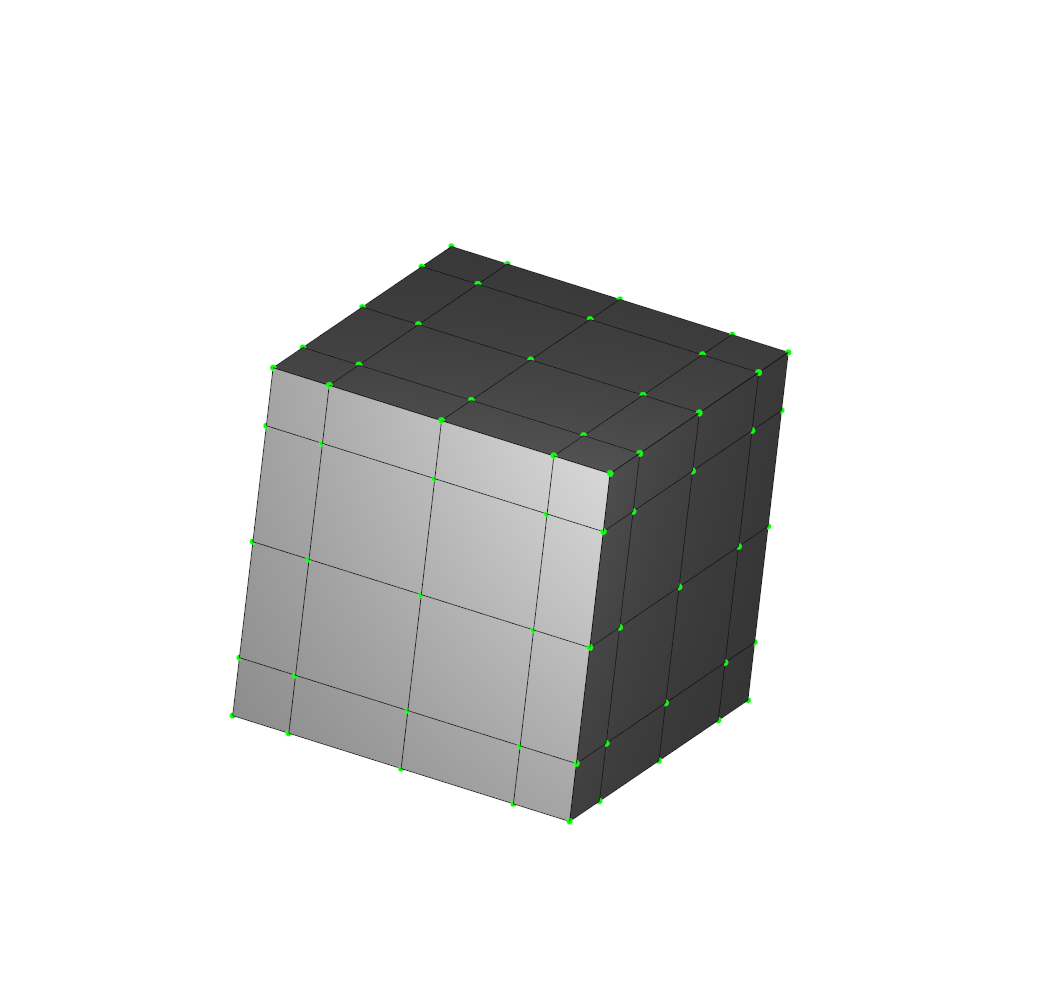
\includegraphics[width=0.31\linewidth]{pic/err0_origin.png}
		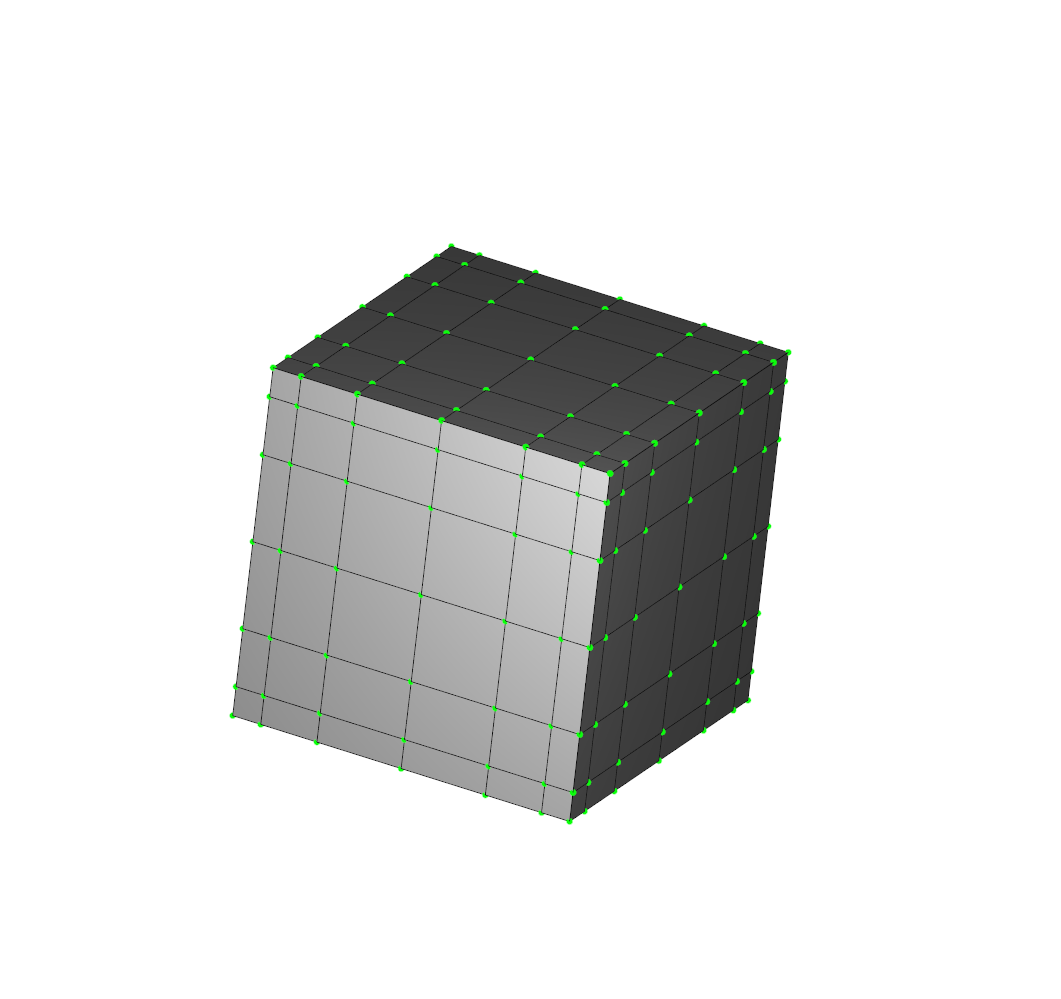
\includegraphics[width=0.31\linewidth]{pic/err5_origin.png}
		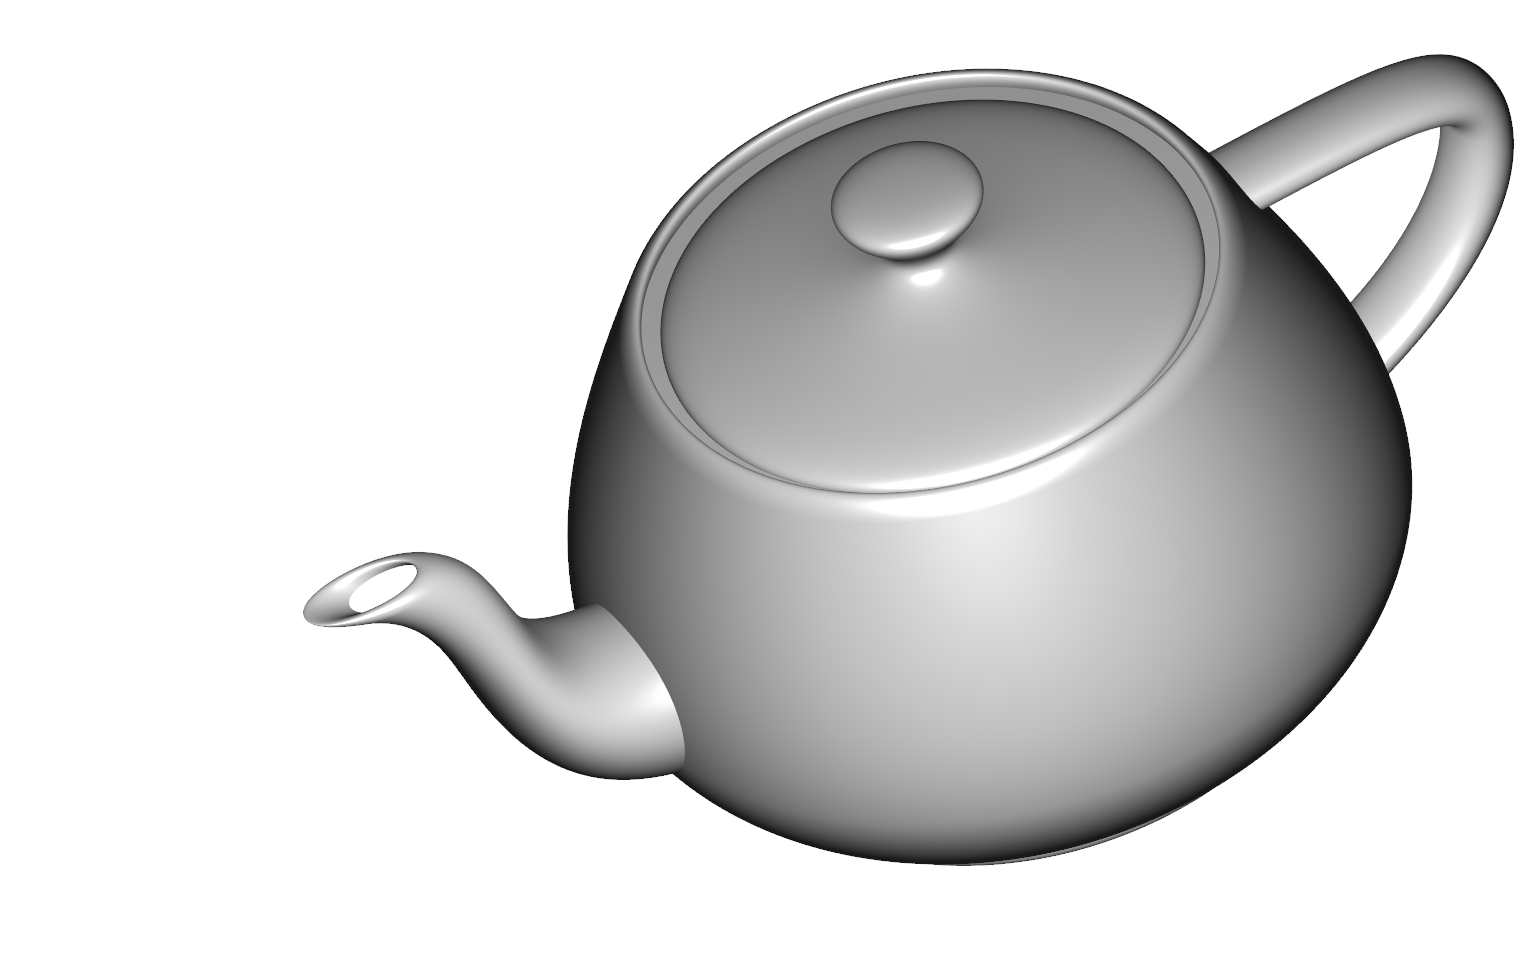
\includegraphics[width=0.31\linewidth]{pic/err12_origin.png}
	}
	\subfigure[\textcolor{red}{Smooth FFD results of (a)}]{
		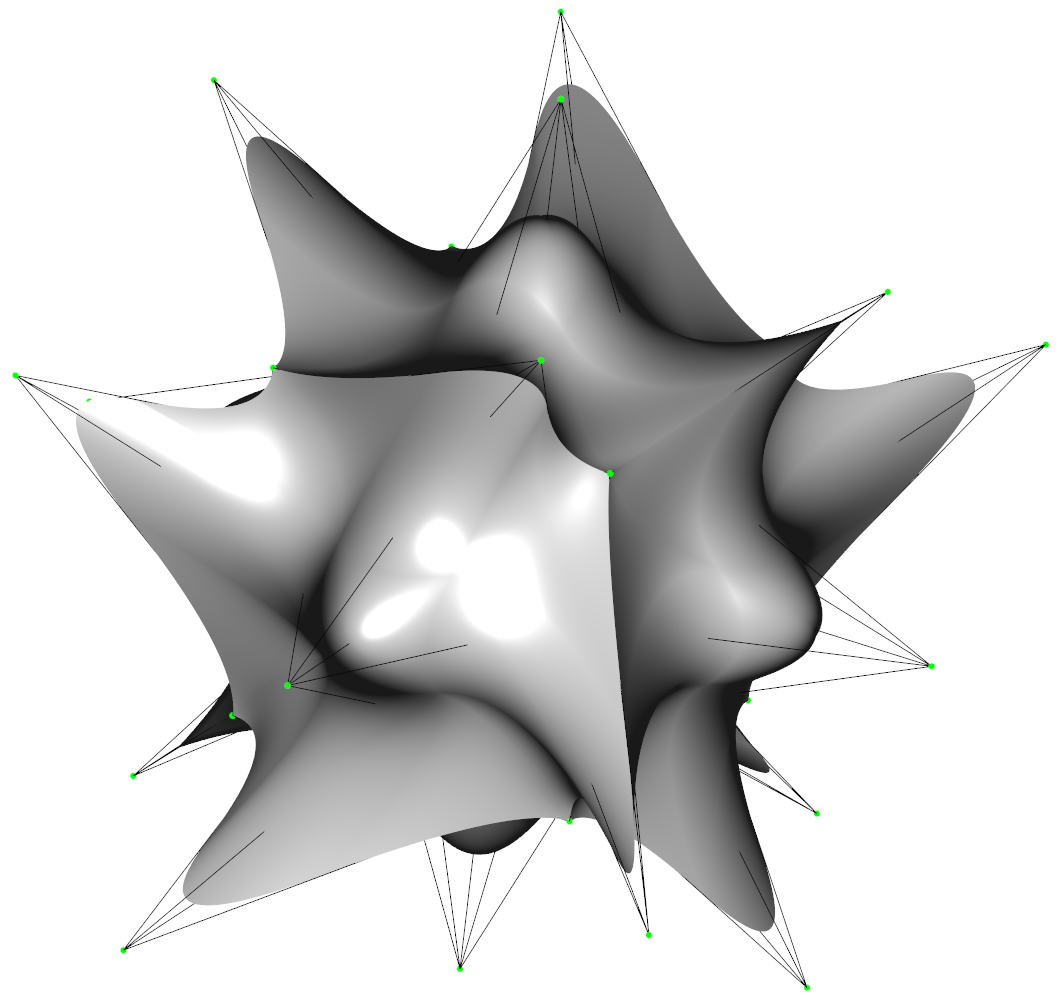
\includegraphics[width=0.31\linewidth]{pic/err1_appro.png}
		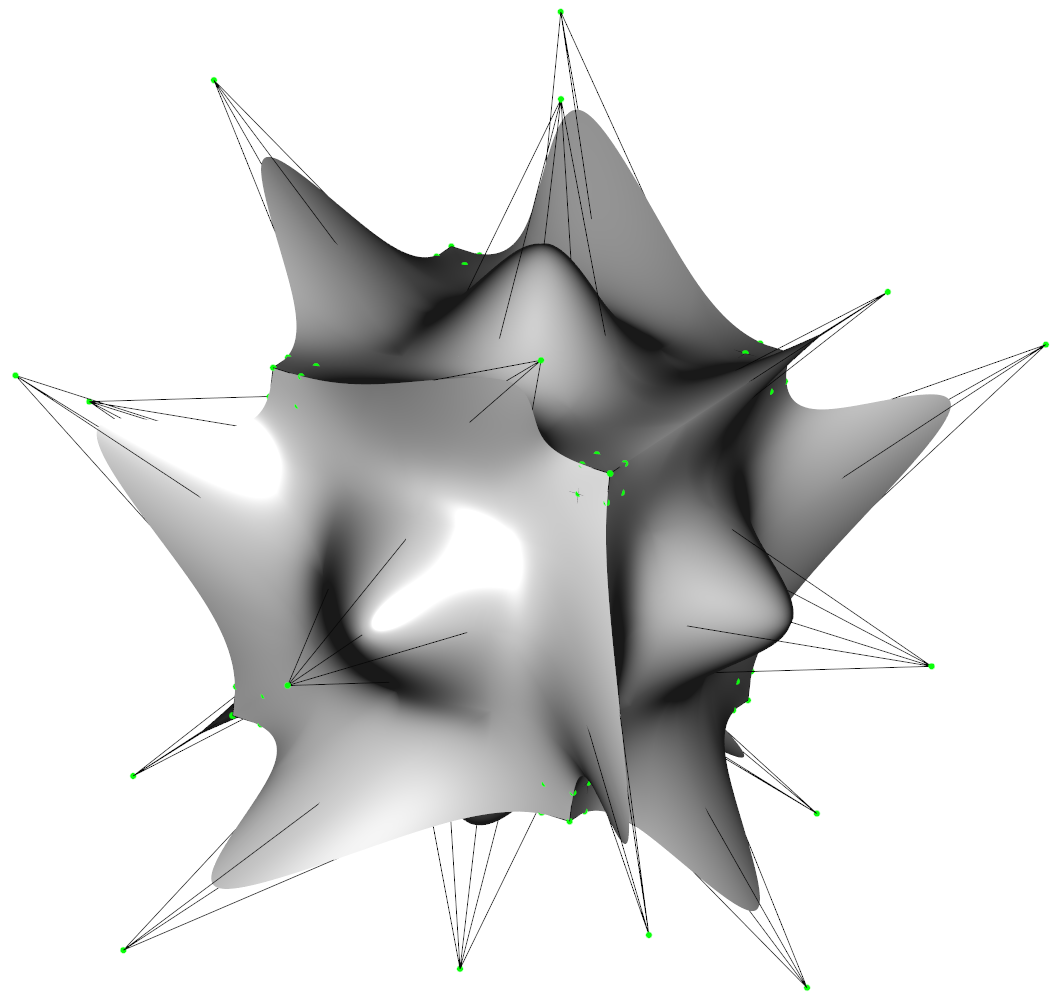
\includegraphics[width=0.31\linewidth]{pic/err6_appro.png}
		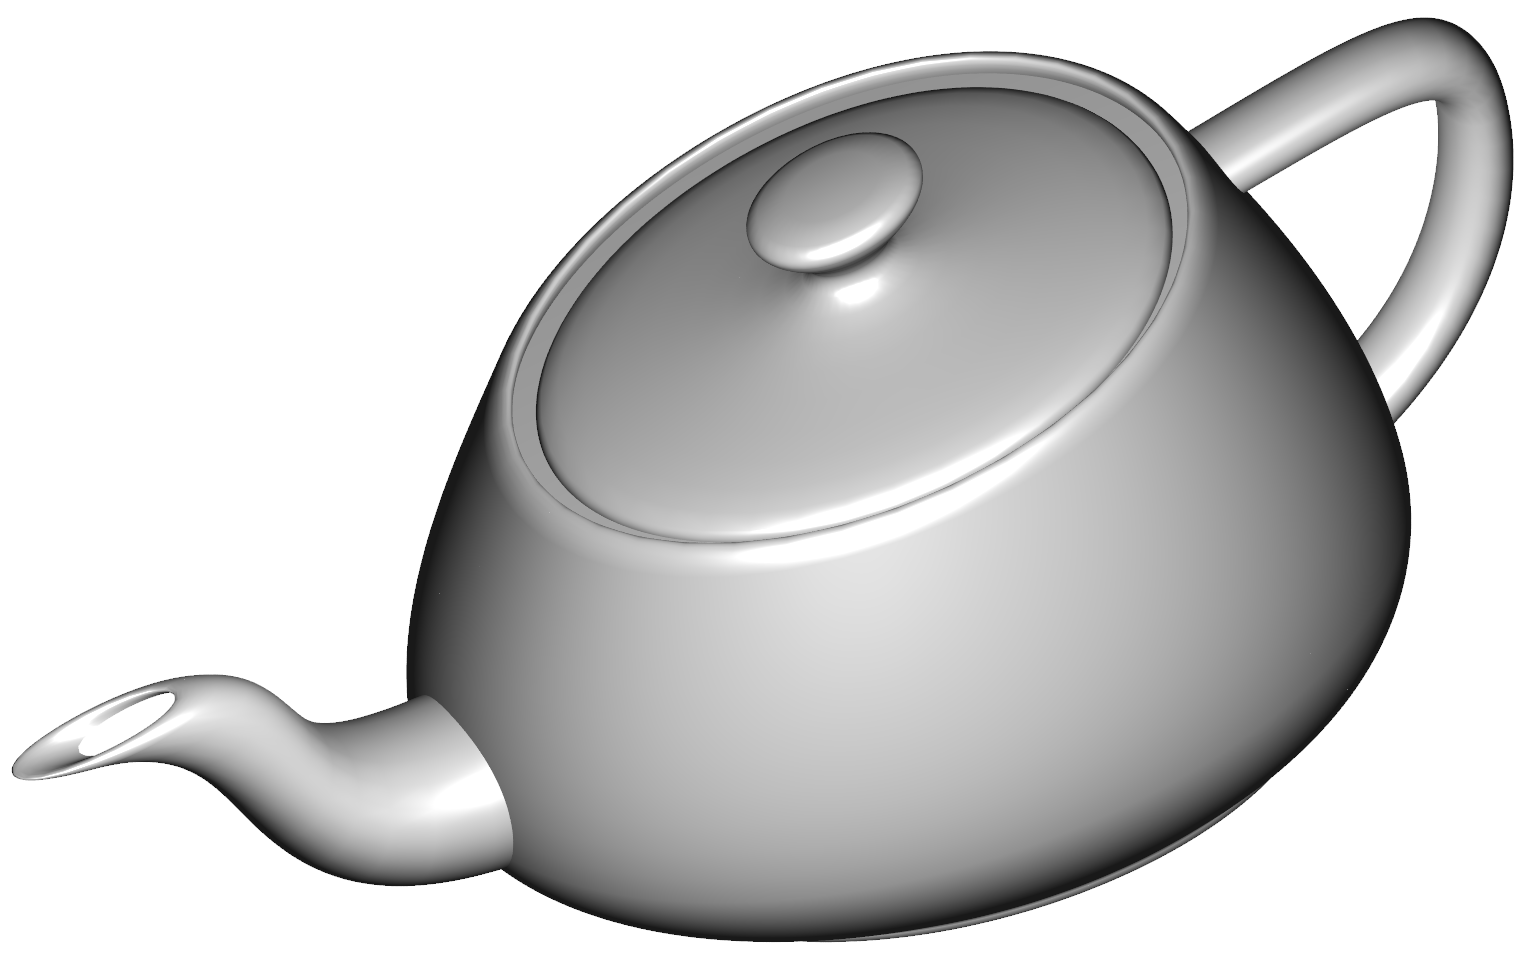
\includegraphics[width=0.31\linewidth]{pic/err13_appro.png}
	}
	\subfigure[\textcolor{red}{Accurate FFD results of (a)}]{
		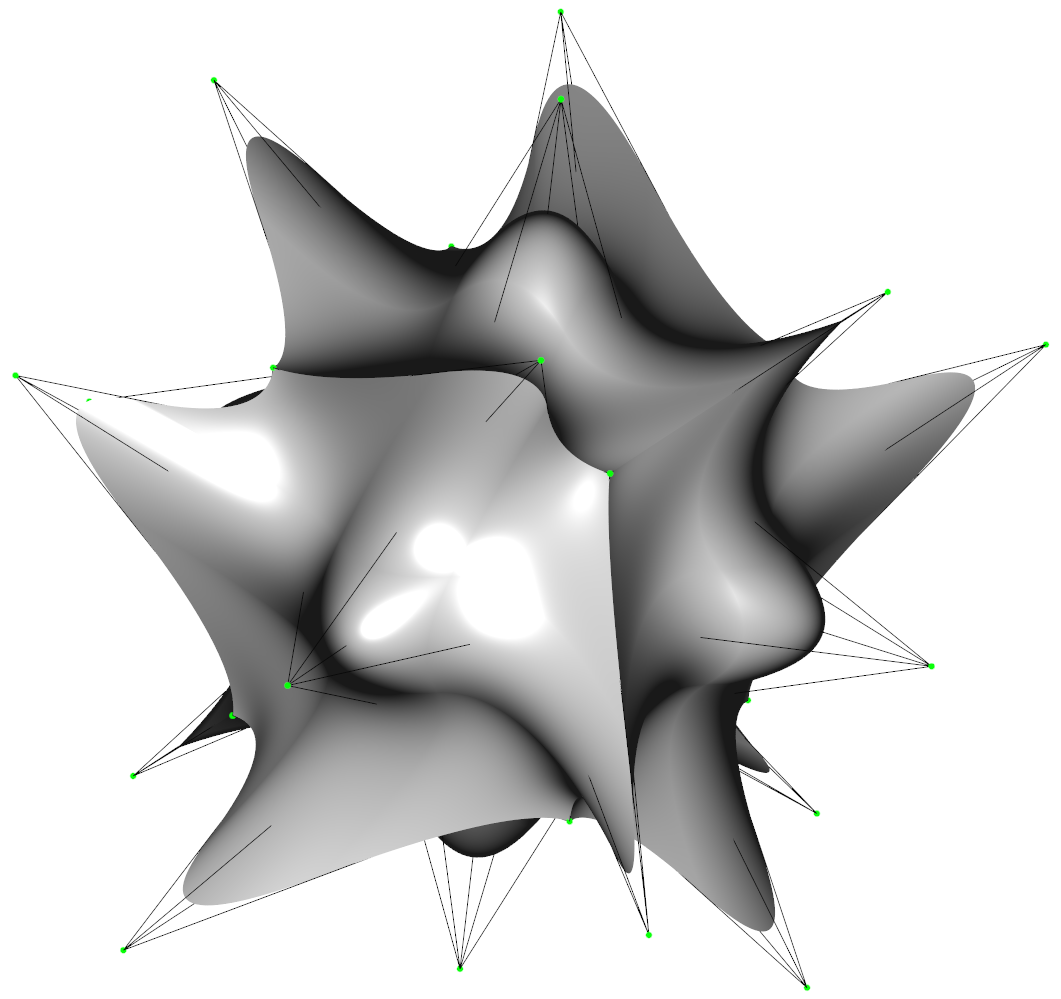
\includegraphics[width=0.31\linewidth]{pic/err2_accu.png}
		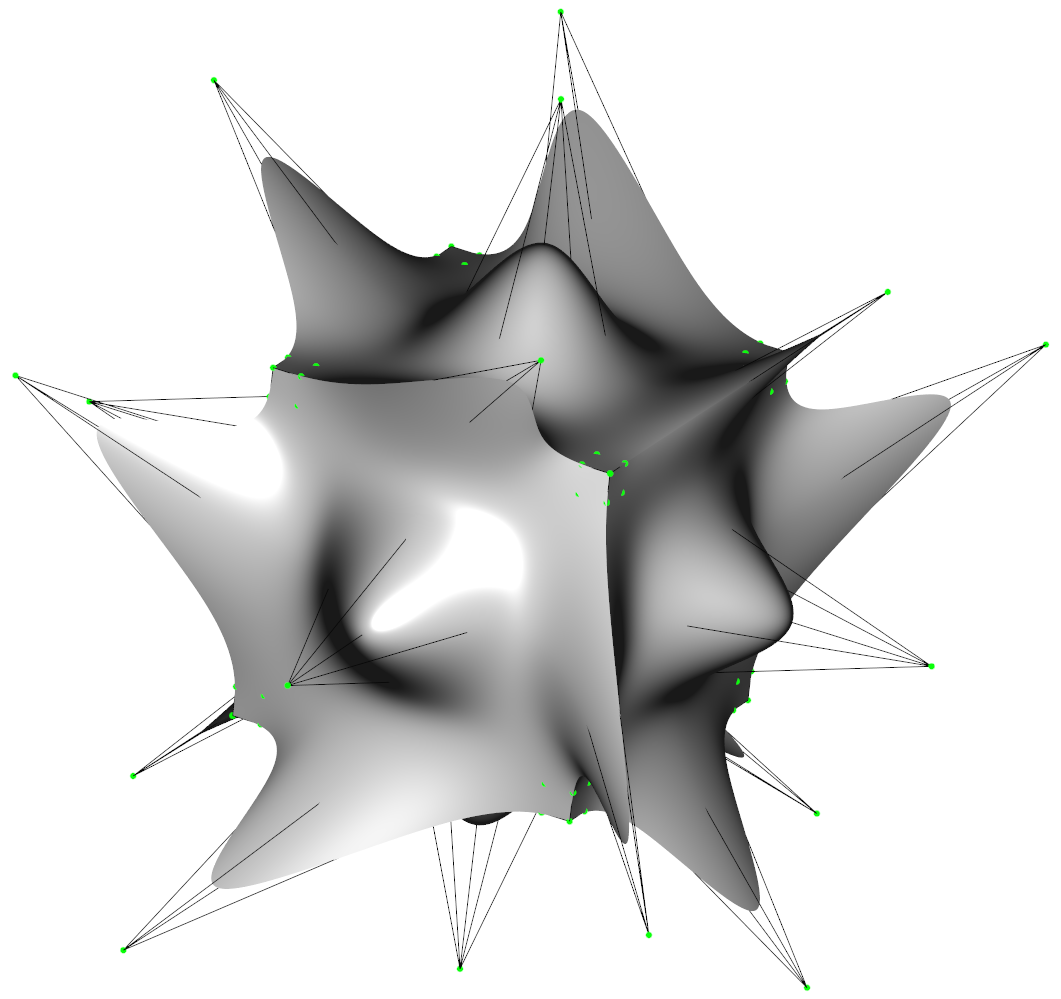
\includegraphics[width=0.31\linewidth]{pic/err7_accu.png}
		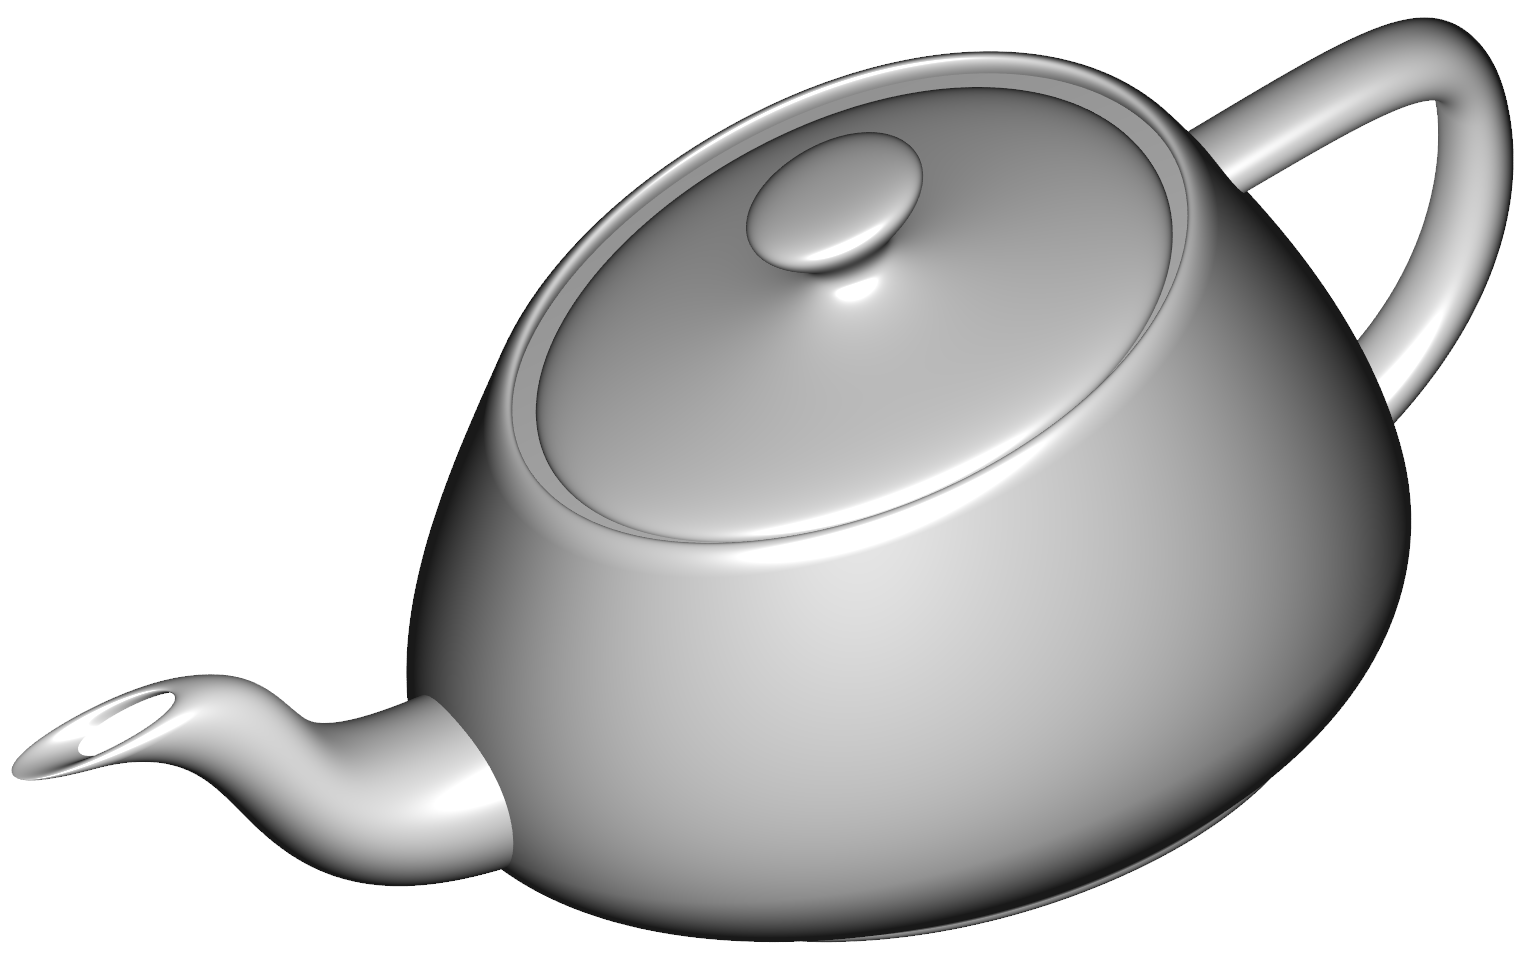
\includegraphics[width=0.31\linewidth]{pic/err14_accu.png}
	}
	\subfigure[\textcolor{red}{Shading differences between (b) and (c)}]{
		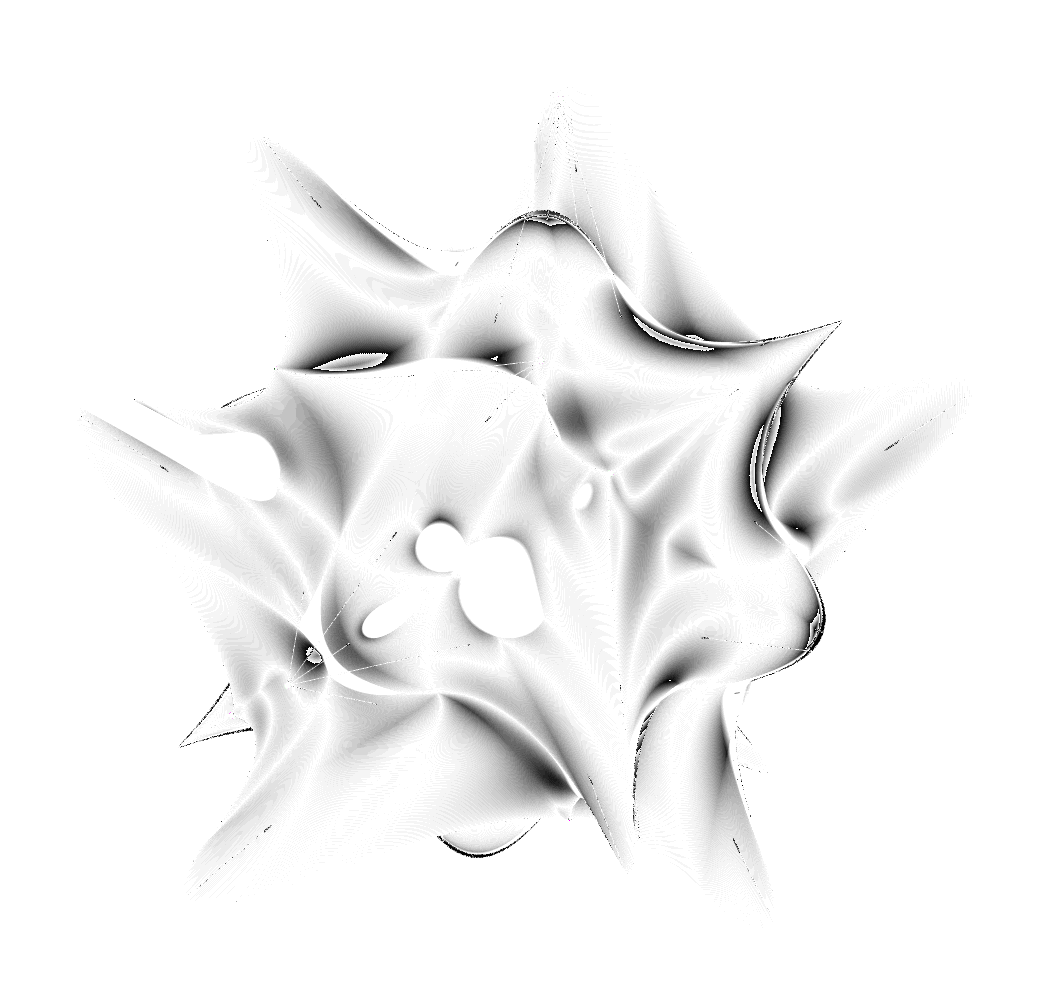
\includegraphics[width=0.31\linewidth]{pic/err10_diff.png}
		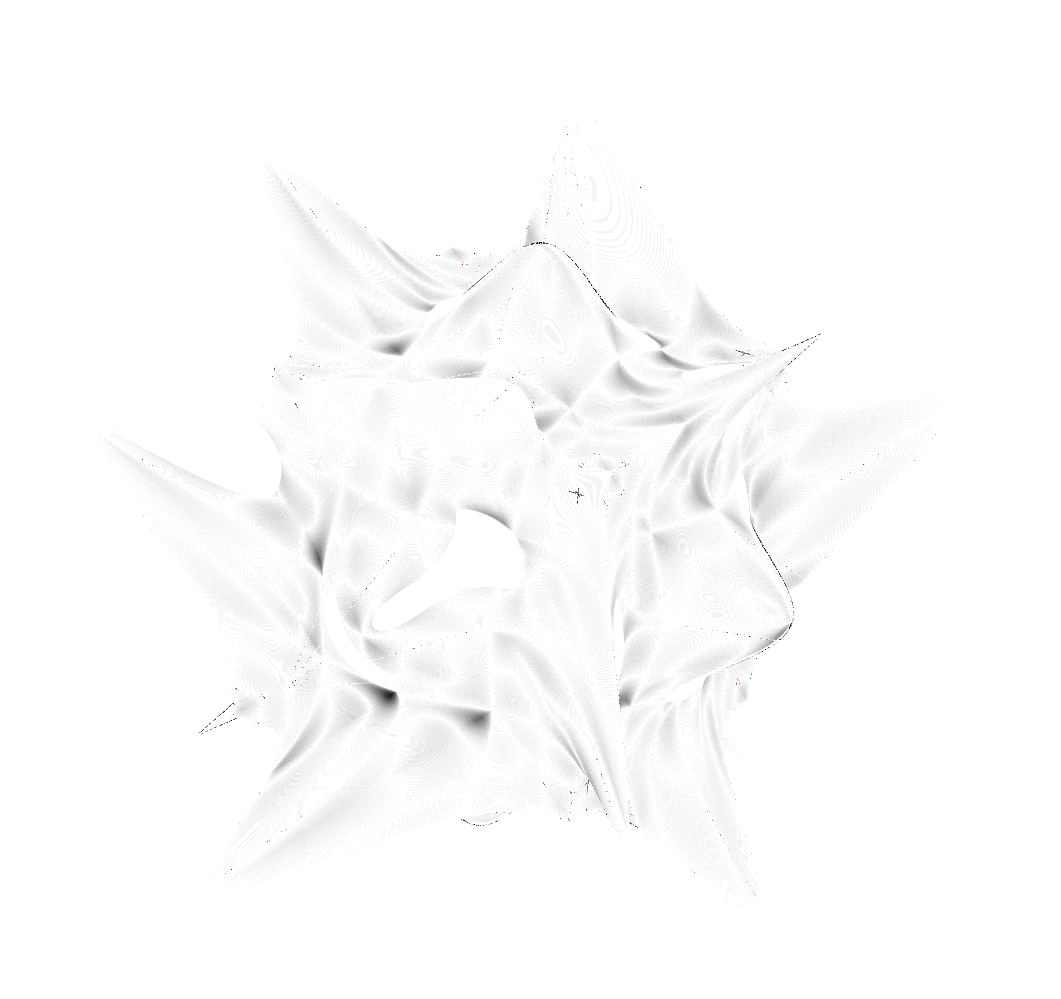
\includegraphics[width=0.31\linewidth]{pic/err11_diff.png}
		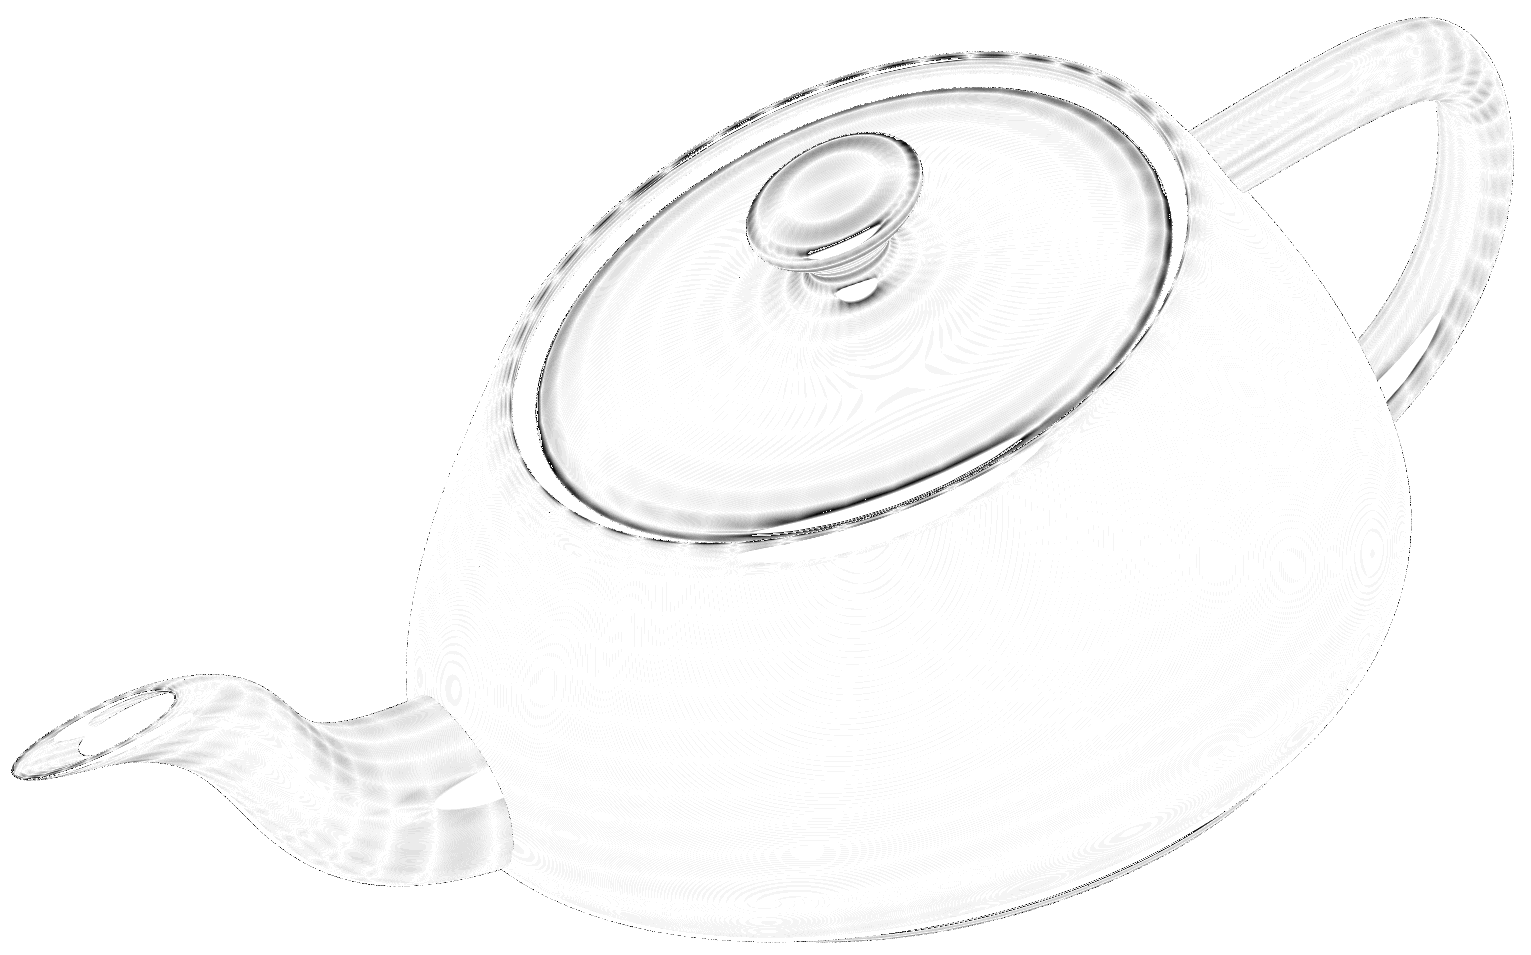
\includegraphics[width=0.31\linewidth]{pic/err17_diff.png}
	}
	\subfigure[\textcolor{red}{Geometry errors}]{
		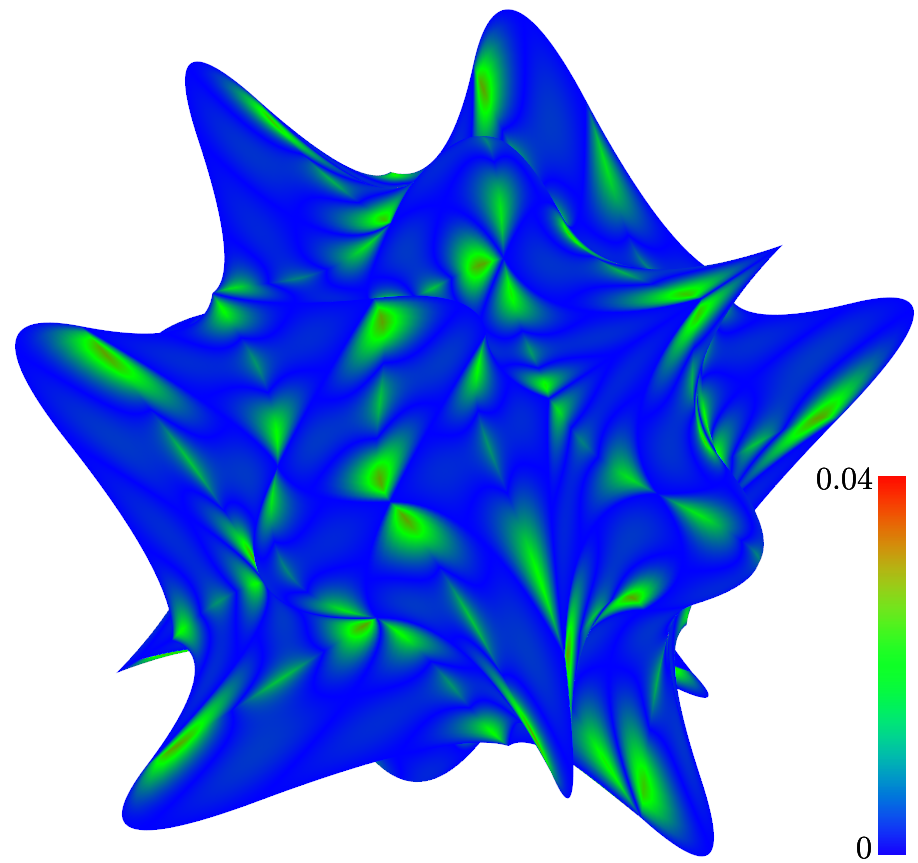
\includegraphics[width=0.31\linewidth]{pic/err3_v.png}
		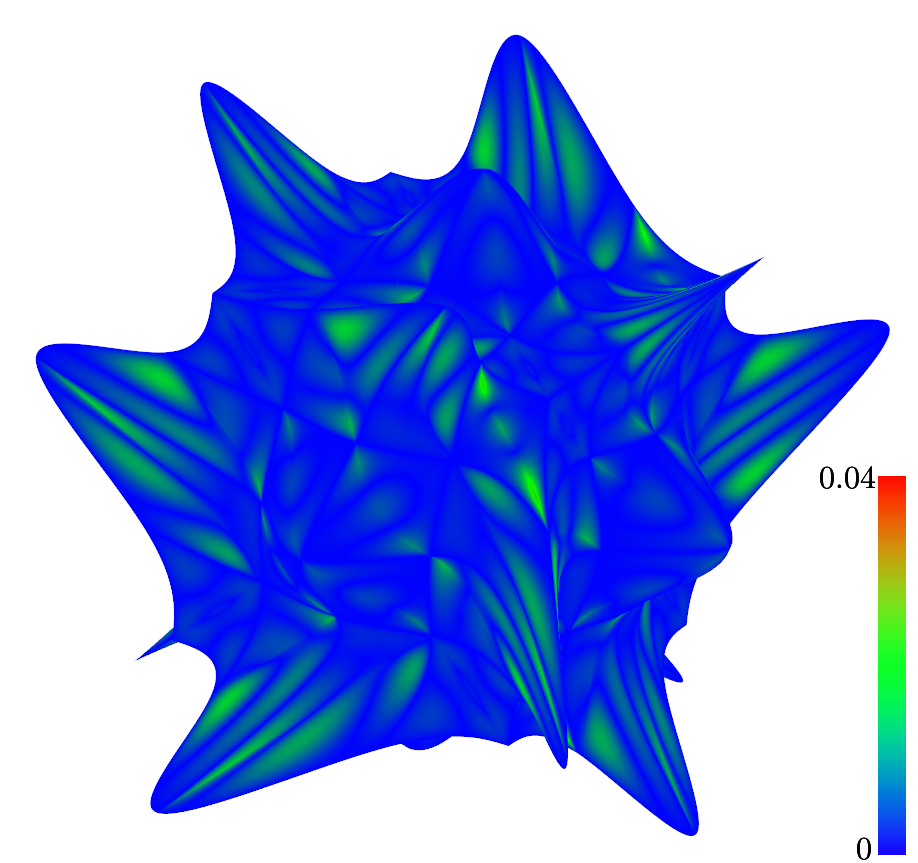
\includegraphics[width=0.31\linewidth]{pic/err8_v.png}
		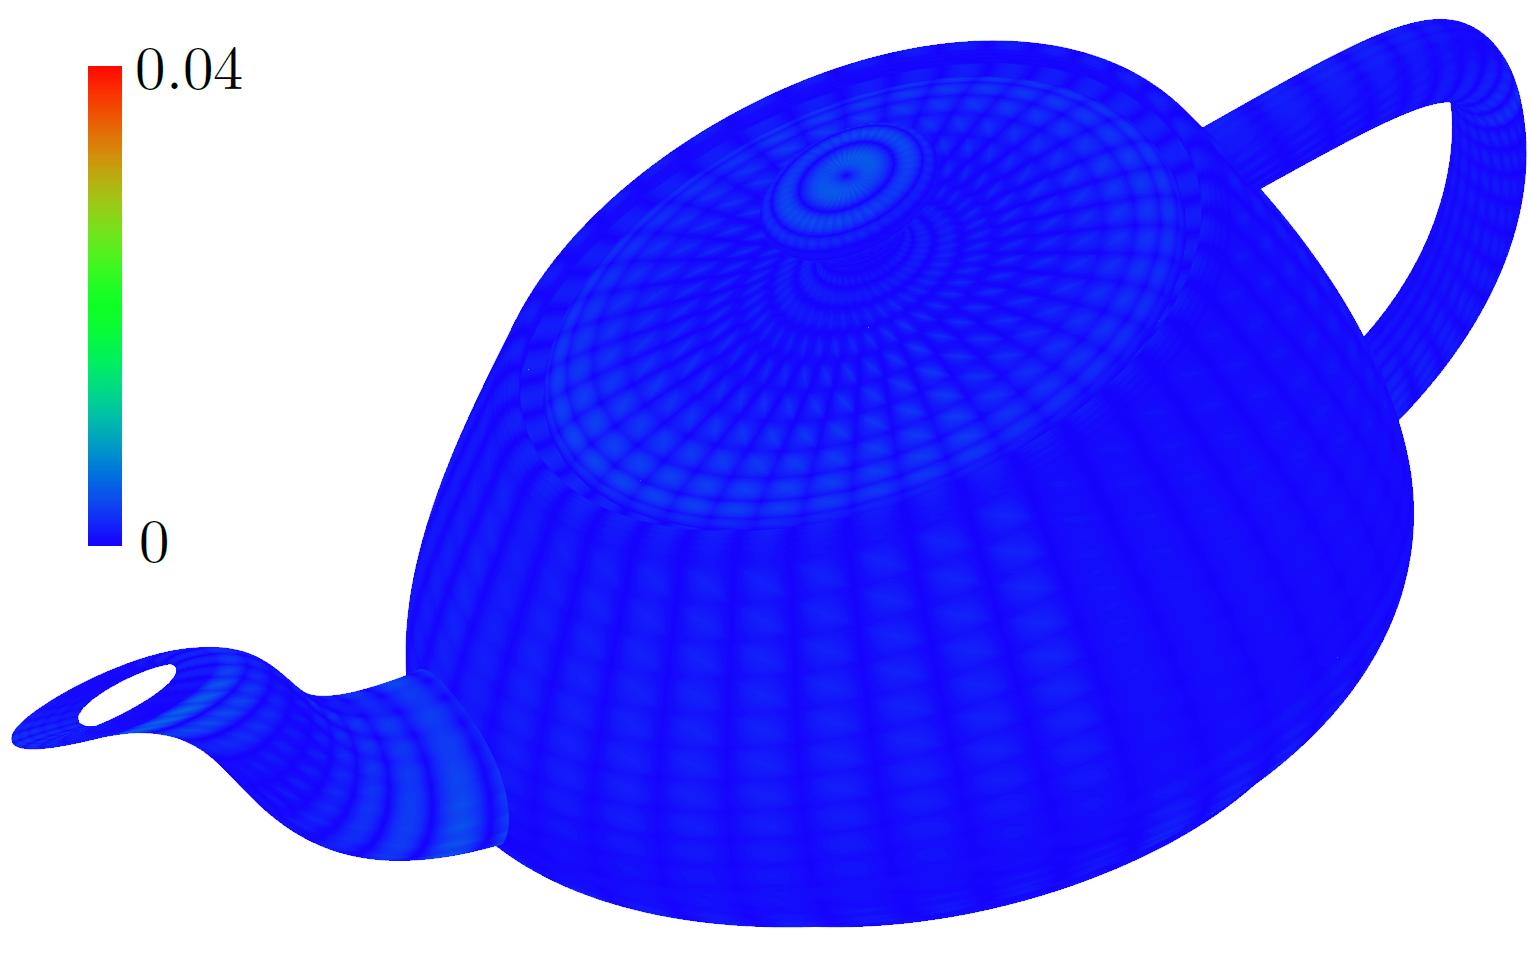
\includegraphics[width=0.31\linewidth]{pic/err15_v.png}
	}
	\subfigure[\textcolor{red}{Normal errors}]{
		\includegraphics[width=0.31\linewidth]{pic/err4_n.png}
		\includegraphics[width=0.31\linewidth]{pic/err9_n.png}
		\includegraphics[width=0.31\linewidth]{pic/err16_n.png}
	}
	\caption{Error testing}
	\label{fig:error}
\end{center}
%\end{figure}
\end{wrapfigure}

In the proposed smooth FFD, both the geometry and normal are obtained approximately via constrained fitting. Thus, there
are approximation errors in the geometry and normal compared with the accurate FFD. Since the smooth parts of a
polygonal object can be regarded as a piecewise linear approximation of a potentially smooth shape, which is unknown in
general, thus it is difficult to evaluate the approximation errors.

Here, we use a Cube model and a Utah teapot model consists of 36 bicubic B\'ezier patches to test the approximation
error, because the geometry and normal of both the input objects are defined accurately. Both of the two models are
normalized into $[-1,1]^3$. The deformations of the Cube model by \cite{Cui13} and \cite{Cui14} are accurate for both
the geometry and normal. The accurate deformation result of Utah teapot is obtained via original FFD of uniformly
sampled points and normals. The input of smooth FFD of the Utah teapot is a mesh generated via de Casteljau
subdivisions. The error test results are shown in Figure~\ref{fig:error}, where the first and second columns are the
Cube model deformed by a $2\times2\times2$ and $3\times3\times3$ B-spline volume, respectively. The third column is the
Utah teapot deformed by a $2\times2\times2$ B-spline volume. \textcolor{red}{For clarity, the shading differences are
inverted and enhanced by 10 times, as shown in Figure~\ref{fig:error}(d).}

The statistics of geometry error, normal error and volume error are given in
Tables~\ref{tab:error_vertex}-\ref{tab:error_volume}, respectively. The geometry error is the Euclidean distances
between the corresponding vertices, and the normal error is the angles between the corresponding normals. The volume
error of Utah teapot is not listed here because it's not a closed model.

According to Figure~\ref{fig:error} and Table~\ref{tab:error_vertex}-\ref{tab:error_volume}, the proposed smooth FFD can
generate good approximations of accurate FFD from the geometry, normal, and volume aspects. Among them, only maximum
normal error of the Utah teapot model is a little bit large. The maximum errors only occur at the spout end and lip
which are high curvature parts. Here the input mesh of the Utah teapot is obtained via uniform sampling approach, thus
it is not a good polygonal approximation to its original smooth model. It leads to the maximum normal approximation
error as above. That is to say the maximum error comes from the polygonal mesh approximation to the smooth object, which
is out of scope of the paper. 

\begin{table}[htbp]
\begin{center}
	\begin{minipage}[c]{0.47\textwidth}
	\footnotesize
	\centering
	\caption{Geometry approximation errors}
	\begin{tabular}{lll}
		\hline
		& Average error & Maximum error \\
		\hline
			Column 1 in Fig.~\ref{fig:error} & 0.00448184 & 0.0274765 \\
			Column 2 in Fig.~\ref{fig:error} & 0.00297672 & 0.0261029 \\
			Column 3 in Fig.~\ref{fig:error} & 0.000906093 & 0.00710446 \\
		\hline
	\end{tabular}
	\label{tab:error_vertex}
	\end{minipage}
	%%%%%%%%%%%%%%%%%%%%%%%%%%%%%%%%%%%%%%%%%%%%%%%%%%%%%%%%%%%
	\begin{minipage}[c]{0.52\textwidth}
	\footnotesize
	\centering
	\caption{Normal approximation errors}
	\begin{tabular}{lll}
		\hline
			& Average error & Maximum error \\
		\hline
			Column 1 in Fig.~\ref{fig:error} & 0.394331$^\circ$ & 4.17587$^\circ$ \\
			Column 2 in Fig.~\ref{fig:error} & 0.387851$^\circ$ & 5.23632$^\circ$ \\
			Column 3 in Fig.~\ref{fig:error} & 0.566609$^\circ$ & 23.3726$^\circ$ \\
		\hline
	\end{tabular}
	\label{tab:error_normal}
	\end{minipage}
\end{center}
\end{table}


\begin{table}[htbp]
	\centering
	\footnotesize
	\caption{Volume approximation errors}
	\begin{tabular}{lllll}
		\hline
			& Degree of the & Model volume after &
			\multirow{2}{*}{Accurate volume($v$)} & \multirow{2}{*}{$\left | v'-v \right| / v$} \\
			& B-spline volume & smooth FFD($v'$) & \multirow{2}{*}{} & \multirow{2}{*}{} \\
		\hline
			%
			\multirow{2}{*}{cube} & $2\times2\times2$ & 16.641 & 16.6449 & 0.023107\% \\
			\multirow{2}{*}{}	  & $3\times3\times3$ & 11.7615 & 11.7651 & 0.0304927\% \\
		\hline
	\end{tabular}
	\label{tab:error_volume}
\end{table}


\subsection{Comparison of smooth FFD and a uniformly upsampling method}

Similar deformation results for polygonal objects can be obtained using a modified GPU-based Uniform UpSampling method
(similar to the UUS method in \cite{Cui13}): step 1: using PN-triangles to replace the triangles in the original object;
step 2: uniformly upsampling the PN-triangles for both the geometry and normal patches; step 3: deform all sampled
points and normals to obtain the deformation result. Here, the Snail model in Figure~\ref{fig:snail:a} is adopted
again. The deformation results are similar because the Snail model consists of lots of small triangles. The runtime
statistics are collected in Table~\ref{tab:uus}. The modified GPU-based UUS method is not as efficient as smooth FFD
when the number of tessellated triangles is relatively large. The rendering times are not considered because they are
the same in both algorithms. This comparison is consistent with the comparison in \cite{Cui13}. However, if the
triangles of the model is relatively large, we can find that the shading of the UUS algorithm is not as good as the
proposed algorithm because the former uses a quadratic normal field on each PN-triangle \cite{Vlachos01}, as shown in
Figure~\ref{fig:uus}.

\begin{figure}[htb] 
  \begin{minipage}[c]{0.66\textwidth} 
	\centering
	\footnotesize
	\tabcaption{Runtime comparison between smooth FFD and modified GPU-based UUS (ms)}
		\begin{tabular}{llll}
			\hline
				Number of sub-triangles & \multirow{2}{*}{Smooth FFD} & \multirow{2}{*}{UUS} &
				\multirow{2}{*}{Smooth FFD/UUS} \\
				in each patch & \multirow{2}{*}{} & \multirow{2}{*}{} & \multirow{2}{*}{} \\
			\hline
				100 & 26.418 & 18.120 & 1.457947 \\
				121 & 27.251 & 21.357 & 1.275975 \\
				144 & 28.954 & 24.859 & 1.164729 \\
				169 & 30.894 & 30.383 & 1.016819 \\
				196 & 31.786 & 34.636 & 0.917716 \\
				225 & 32.773 & 39.224 & 0.835534 \\
				256 & 36.183 & 44.120 & 0.820104 \\
			\hline
		\end{tabular}
	\label{tab:uus}
  \end{minipage} 
  %%%%%%%%%%%%%%%%%%%%%%%%%%%%%%%%%%%%%%%%%%%%%%%%%%%%%%%%%%%%%%%%%%%
  \begin{minipage}[c]{0.33\textwidth} 
		\centering
		\subfigure[]{\includegraphics[width=0.46\linewidth]{pic/uus1.png}}
		\subfigure[]{\includegraphics[width=0.46\linewidth]{pic/uus2.png}}
		\caption{Shading results for smooth FFD (a) and UUS algorithm (b). Each B\'ezier patch is
		tessellated into 100 sub-triangles.}
		\label{fig:uus}
  \end{minipage}% 
\end{figure}


\subsection{Comparison of smooth FFD and an adaptive tessellation shader method}

Tessellation shader which has been added to OpenGL since version 4.0 is a suitable tool to tessellate the generated
cubic triangular B\'ezier surface patches. So, we also implemented an adaptive tessellation of cubic triangular patches
using tessellation shader. The tessellation factors of three edges of a patch are proportional to their lengths. This
adaptive approach shares the same steps with smooth FFD until the control points of all cubic triangular B\'ezier
patches are obtained. After that, the adaptive tessellation shader method is performed to render these patches directly,
while the smooth FFD will calculate the tessellation points by cuBLAS first, then copy the result to OpenGL VBO, and
render the sub-triangles finally.

\begin{wrapfigure}{r}{0.40\textwidth}
%\begin{figure}[htbp]
	\centering
		\centering
		\subfigure[Adaptive tessellation]{\includegraphics[width=0.45\linewidth]{pic/granularity1.png}}
		\subfigure[Smooth FFD]{\includegraphics[width=0.48\linewidth]{pic/granularity2.png}}
		\caption{Comparison of tessellation granularity}
		\label{fig:granularity}
%\end{figure}
\end{wrapfigure}

The Vase model shown in Figure~\ref{fig:all_ffd} is adopted as the test example. The tessellation granularities of two
methods are shown in Figure~\ref{fig:granularity}. In the tessellation shader method, the longest edge are tessellated
into 27 segments. For fair comparison, in the smooth FFD, all the edges are tessellated uniformly into 27 segments. The
time comparison of them is shown in Table~\ref{tab:adaptive_tess}. As we can see, the efficiency of the tessellation
shader method is not as efficient as that of the smooth FFD. The main reason is that the smooth FFD is a perfect SIMD
task, it can make full use of the GPU streaming processors. Of course, if the object is composed of tiny, slim and large
triangles, it is possible that the adaptive tessellation approach may perform better than the uniform tessellation.

\begin{table}[htbp]
	\centering
	\footnotesize
	\caption{Comparison of the times for the smooth FFD and adaptive tessellation shader method (ms)}
		\begin{tabular}{lll}
			\hline
			& Smooth FFD & Tess shader method \\
			\hline
			Calculate the tess points	& 0.456 & -  \\
			Copy results to the VBO		& 0.576 & -  \\
			Render						& 3.031 & 6.082  \\
			Total						& 4.063 & 6.082  \\
			\hline
		\end{tabular}
	\label{tab:adaptive_tess}
\end{table}

%%%%%%%%%%%%%%%%%%%%%%%%%%%%%%%%%%%%%%%%%%%%%%%%%%%%%%%%%%%%%%%%%%%%

\section{Conclusion and Future Work}

In this paper, we proposed a GPU-based smooth FFD with sharp features awareness that addresses the unsmoothness of the
normal field and the geometry artifact problems in the framework of accurate FFD. The algorithm can produce a
high-quality deformation result. It is a highly parallellizable GPU algorithm and is able to deform a relatively
large-scale model in real time. The algorithm is intuitive and can be implemented easily. It can handle relatively
coarse meshes and generate smooth deformation results.

The approach can still be improved in several aspects. First, the uniform tessellation of the cubic triangular B\'ezier
patches will generate many unnecessary small triangles. An efficient adaptive tessellation algorithm via GPGPU is an
alternative to our method. Second, the approximation error of the smooth FFD for polygonal object is worth to be
analyzed in theory. A feasible error bound is useful to guide the discretization of an smooth object, which is essential
for generating high-quality deformation result.

\section{Acknowledgement}

\textcolor{red}{
The authors would like to thank the anonymous reviewers who gave valuable suggestions to improve the quality of the
paper. This work was supported by the National Natural Science Foundation of China under Grant Nos. 61170138 and
61472349.
}

\section*{References}

\bibliography{MyBib}

\end{document}
